% This is the Reed College LaTeX thesis template. Most of the work
% for the document class was done by Sam Noble (SN), as well as this
% template. Later comments etc. by Ben Salzberg (BTS). Additional
% restructuring and APA support by Jess Youngberg (JY).
% Your comments and suggestions are more than welcome; please email
% them to cus@reed.edu
%
% See https://www.reed.edu/cis/help/LaTeX/index.html for help. There are a
% great bunch of help pages there, with notes on
% getting started, bibtex, etc. Go there and read it if you're not
% already familiar with LaTeX.
%
% Any line that starts with a percent symbol is a comment.
% They won't show up in the document, and are useful for notes
% to yourself and explaining commands.
% Commenting also removes a line from the document;
% very handy for troubleshooting problems. -BTS

% As far as I know, this follows the requirements laid out in
% the 2002-2003 Senior Handbook. Ask a librarian to check the
% document before binding. -SN

%%
%% Preamble
%%
% \documentclass{<something>} must begin each LaTeX document
\documentclass[12pt,twoside]{reedthesis}
% Packages are extensions to the basic LaTeX functions. Whatever you
% want to typeset, there is probably a package out there for it.
% Chemistry (chemtex), screenplays, you name it.
% Check out CTAN to see: https://www.ctan.org/
%%
\usepackage{graphicx,latexsym}
\usepackage{amsmath}
\usepackage{amssymb,amsthm}
\usepackage{longtable,booktabs,setspace}
\usepackage{chemarr} %% Useful for one reaction arrow, useless if you're not a chem major
\usepackage[hyphens]{url}
% Added by CII
\usepackage{hyperref}
\usepackage{lmodern}
\usepackage{float}
\floatplacement{figure}{H}
% Thanks, @Xyv
\usepackage{calc}
% End of CII addition
\usepackage{rotating}

% Next line commented out by CII
%%% \usepackage{natbib}
% Comment out the natbib line above and uncomment the following two lines to use the new
% biblatex-chicago style, for Chicago A. Also make some changes at the end where the
% bibliography is included.
%\usepackage{biblatex-chicago}
%\bibliography{thesis}


% Added by CII (Thanks, Hadley!)
% Use ref for internal links
\renewcommand{\hyperref}[2][???]{\autoref{#1}}
\def\chapterautorefname{Chapter}
\def\sectionautorefname{Section}
\def\subsectionautorefname{Subsection}
% End of CII addition

% Added by CII
\usepackage{caption}
\captionsetup{width=5in}
% End of CII addition

% \usepackage{times} % other fonts are available like times, bookman, charter, palatino

% Syntax highlighting #22
  \usepackage{color}
  \usepackage{fancyvrb}
  \newcommand{\VerbBar}{|}
  \newcommand{\VERB}{\Verb[commandchars=\\\{\}]}
  \DefineVerbatimEnvironment{Highlighting}{Verbatim}{commandchars=\\\{\}}
  % Add ',fontsize=\small' for more characters per line
  \usepackage{framed}
  \definecolor{shadecolor}{RGB}{248,248,248}
  \newenvironment{Shaded}{\begin{snugshade}}{\end{snugshade}}
  \newcommand{\AlertTok}[1]{\textcolor[rgb]{0.94,0.16,0.16}{#1}}
  \newcommand{\AnnotationTok}[1]{\textcolor[rgb]{0.56,0.35,0.01}{\textbf{\textit{#1}}}}
  \newcommand{\AttributeTok}[1]{\textcolor[rgb]{0.77,0.63,0.00}{#1}}
  \newcommand{\BaseNTok}[1]{\textcolor[rgb]{0.00,0.00,0.81}{#1}}
  \newcommand{\BuiltInTok}[1]{#1}
  \newcommand{\CharTok}[1]{\textcolor[rgb]{0.31,0.60,0.02}{#1}}
  \newcommand{\CommentTok}[1]{\textcolor[rgb]{0.56,0.35,0.01}{\textit{#1}}}
  \newcommand{\CommentVarTok}[1]{\textcolor[rgb]{0.56,0.35,0.01}{\textbf{\textit{#1}}}}
  \newcommand{\ConstantTok}[1]{\textcolor[rgb]{0.00,0.00,0.00}{#1}}
  \newcommand{\ControlFlowTok}[1]{\textcolor[rgb]{0.13,0.29,0.53}{\textbf{#1}}}
  \newcommand{\DataTypeTok}[1]{\textcolor[rgb]{0.13,0.29,0.53}{#1}}
  \newcommand{\DecValTok}[1]{\textcolor[rgb]{0.00,0.00,0.81}{#1}}
  \newcommand{\DocumentationTok}[1]{\textcolor[rgb]{0.56,0.35,0.01}{\textbf{\textit{#1}}}}
  \newcommand{\ErrorTok}[1]{\textcolor[rgb]{0.64,0.00,0.00}{\textbf{#1}}}
  \newcommand{\ExtensionTok}[1]{#1}
  \newcommand{\FloatTok}[1]{\textcolor[rgb]{0.00,0.00,0.81}{#1}}
  \newcommand{\FunctionTok}[1]{\textcolor[rgb]{0.00,0.00,0.00}{#1}}
  \newcommand{\ImportTok}[1]{#1}
  \newcommand{\InformationTok}[1]{\textcolor[rgb]{0.56,0.35,0.01}{\textbf{\textit{#1}}}}
  \newcommand{\KeywordTok}[1]{\textcolor[rgb]{0.13,0.29,0.53}{\textbf{#1}}}
  \newcommand{\NormalTok}[1]{#1}
  \newcommand{\OperatorTok}[1]{\textcolor[rgb]{0.81,0.36,0.00}{\textbf{#1}}}
  \newcommand{\OtherTok}[1]{\textcolor[rgb]{0.56,0.35,0.01}{#1}}
  \newcommand{\PreprocessorTok}[1]{\textcolor[rgb]{0.56,0.35,0.01}{\textit{#1}}}
  \newcommand{\RegionMarkerTok}[1]{#1}
  \newcommand{\SpecialCharTok}[1]{\textcolor[rgb]{0.00,0.00,0.00}{#1}}
  \newcommand{\SpecialStringTok}[1]{\textcolor[rgb]{0.31,0.60,0.02}{#1}}
  \newcommand{\StringTok}[1]{\textcolor[rgb]{0.31,0.60,0.02}{#1}}
  \newcommand{\VariableTok}[1]{\textcolor[rgb]{0.00,0.00,0.00}{#1}}
  \newcommand{\VerbatimStringTok}[1]{\textcolor[rgb]{0.31,0.60,0.02}{#1}}
  \newcommand{\WarningTok}[1]{\textcolor[rgb]{0.56,0.35,0.01}{\textbf{\textit{#1}}}}

% To pass between YAML and LaTeX the dollar signs are added by CII
\title{Optimizing Lempel Ziv Welch for DNA Compression}
\author{Caden Corontzos}
% The month and year that you submit your FINAL draft TO THE LIBRARY (May or December)
\date{May 2023}
\division{Mathematics and Natural Sciences}
\advisor{Eitan Frachtenberg}
\institution{Reed College}
\degree{Bachelor of Arts}
%If you have two advisors for some reason, you can use the following
% Uncommented out by CII
% End of CII addition

%%% Remember to use the correct department!
\department{Computer Science}
% if you're writing a thesis in an interdisciplinary major,
% uncomment the line below and change the text as appropriate.
% check the Senior Handbook if unsure.
%\thedivisionof{The Established Interdisciplinary Committee for}
% if you want the approval page to say "Approved for the Committee",
% uncomment the next line
%\approvedforthe{Committee}

% Added by CII
%%% Copied from knitr
%% maxwidth is the original width if it's less than linewidth
%% otherwise use linewidth (to make sure the graphics do not exceed the margin)
\makeatletter
\def\maxwidth{ %
  \ifdim\Gin@nat@width>\linewidth
    \linewidth
  \else
    \Gin@nat@width
  \fi
}
\makeatother

% From {rticles}
\newlength{\csllabelwidth}
\setlength{\csllabelwidth}{3em}
\newlength{\cslhangindent}
\setlength{\cslhangindent}{1.5em}
% for Pandoc 2.8 to 2.10.1
\newenvironment{cslreferences}%
  {}%
  {\par}
% For Pandoc 2.11+
% As noted by @mirh [2] is needed instead of [3] for 2.12
\newenvironment{CSLReferences}[2] % #1 hanging-ident, #2 entry spacing
 {% don't indent paragraphs
  \setlength{\parindent}{0pt}
  % turn on hanging indent if param 1 is 1
  \ifodd #1 \everypar{\setlength{\hangindent}{\cslhangindent}}\ignorespaces\fi
  % set entry spacing
  \ifnum #2 > 0
  \setlength{\parskip}{#2\baselineskip}
  \fi
 }%
 {}
\usepackage{calc} % for calculating minipage widths
\newcommand{\CSLBlock}[1]{#1\hfill\break}
\newcommand{\CSLLeftMargin}[1]{\parbox[t]{\csllabelwidth}{#1}}
\newcommand{\CSLRightInline}[1]{\parbox[t]{\linewidth - \csllabelwidth}{#1}}
\newcommand{\CSLIndent}[1]{\hspace{\cslhangindent}#1}

\renewcommand{\contentsname}{Table of Contents}
% End of CII addition

\setlength{\parskip}{0pt}

% Added by CII

\providecommand{\tightlist}{%
  \setlength{\itemsep}{0pt}\setlength{\parskip}{0pt}}

\Acknowledgements{
I want to thank a few people.
}

\Dedication{
You can have a dedication here if you wish.
}

\Preface{
This is an example of a thesis setup to use the reed thesis document class
(for LaTeX) and the R bookdown package, in general.
}

\Abstract{
The Lempel Ziv Welch compression algorithm is a lossless data compression algorithm used for numerous applications, including the Unix file compression utility \texttt{compress} and the GIF image format. Storing, reading, and transferring enormous amounts of data is often an issue in the biological field, especially when concerning DNA. This thesis explores the application of Lempel Ziv Welch to the compression of DNA. A variety of different optimization of the original LZW algorithm are explore included palatalizing, multiple dictionaries, and some other cool thing here broh.
}

	\usepackage{setspace}\onehalfspacing
\usepackage[edges]{forest}
\usepackage{tikz}
	\usepackage{forest}
\usepackage{tikz}
\usepackage{booktabs}
\usepackage{longtable}
\usepackage{array}
\usepackage{multirow}
\usepackage{wrapfig}
\usepackage{float}
\usepackage{colortbl}
\usepackage{pdflscape}
\usepackage{tabu}
\usepackage{threeparttable}
\usepackage{threeparttablex}
\usepackage[normalem]{ulem}
\usepackage{makecell}
\usepackage{xcolor}
% End of CII addition
%%
%% End Preamble
%%
%
\begin{document}

% Everything below added by CII
  \maketitle

\frontmatter % this stuff will be roman-numbered
\pagestyle{empty} % this removes page numbers from the frontmatter
  \begin{acknowledgements}
    I want to thank a few people.
  \end{acknowledgements}
  \begin{preface}
    This is an example of a thesis setup to use the reed thesis document class
    (for LaTeX) and the R bookdown package, in general.
  \end{preface}
\chapter*{List of Abbreviations}
\begin{table}[h]
    \centering
    \begin{tabular}{ll}
                \textbf{LZW} & Lempel Ziv Welch \\
            \end{tabular}
\end{table}
  \hypersetup{linkcolor=black}
  \setcounter{secnumdepth}{2}
  \setcounter{tocdepth}{2}
  \tableofcontents

  \listoftables

  \listoffigures
  \begin{abstract}
    The Lempel Ziv Welch compression algorithm is a lossless data compression algorithm used for numerous applications, including the Unix file compression utility \texttt{compress} and the GIF image format. Storing, reading, and transferring enormous amounts of data is often an issue in the biological field, especially when concerning DNA. This thesis explores the application of Lempel Ziv Welch to the compression of DNA. A variety of different optimization of the original LZW algorithm are explore included palatalizing, multiple dictionaries, and some other cool thing here broh.
  \end{abstract}
  \begin{dedication}
    You can have a dedication here if you wish.
  \end{dedication}
\mainmatter % here the regular arabic numbering starts
\pagestyle{fancyplain} % turns page numbering back on

\hypertarget{introduction}{%
\chapter*{Introduction}\label{introduction}}
\addcontentsline{toc}{chapter}{Introduction}

When dealing with DNA, it

\hypertarget{backround-and-motivations}{%
\chapter{Backround and Motivations}\label{backround-and-motivations}}

This thesis deals with some high level topics and uses language specific to compression research. This chapter tries to give brief summaries and examples of the relevant topics to be discussed so readers of all experience levels can put our results into context.

\hypertarget{what-is-information}{%
\section{What is information?}\label{what-is-information}}

Suppose you had an idea that you wanted to share with another person. Humans have many ways to communicate information; you could send a text message, you could tell them with words, you could tell them with sign language. But regardless of the medium, you have some idea that you want to get across. Does it matter if the other person gets your message exactly? Or can it be part of the message? If someone asks you ``Where library'', despite the lack of prepositions you still understand what they mean. So did that person convey any less information than a person who asks ``Where is the library?''
Clearly, information is fundamental to how humans interact and how they understand the world, but defining it proves difficult. For our purposes, let us assume that information is something that can be interpreted to glean information that you didn't know before.

Information on computers can take many forms, such as text, audio, and video. This information can travel through many channels including the internet, wires, screens, etc. To maximize the amount of information that can be transmitted through a channel, we need to encode the information in a way which minimizes its size, while also preserving its essential features. This process is called compression.

\hypertarget{compression-a-history}{%
\section{Compression: A history}\label{compression-a-history}}

The idea of compressing data to make transmission easier has been around for a long time. One of the earliest uses of compression was the use of Morse code, developed by Samuel Morse in the 1830s, used to transmit messages over telegraph. Morse uses a binary code, where dots and dashes represent different letters and numbers of the message to be transmitted.

In the 1970s, researchers began to develop more sophisticated compression algoritms, such as Huffman encoding and Lempel-Ziv compression. Both LZW and Huffman use codes to represent different characters in a message.

TODO: Elaborate
\#\# Compression Metrics

\hypertarget{compression-ratio}{%
\subsection{Compression Ratio}\label{compression-ratio}}

Compression Ratio is the measure of size reduction achieved by a compression algorithm. It is typically expressd as a ratio of the size of the uncompressed data (\(OS\)) to the size of the compressed data (\{CS\}).

\[CR = \frac{OS}{CS}\]

So a higher compression ratio means a more effective compression algorithm, and means that we were able to store more data in less space, allowing for easier storage and transfer.

\hypertarget{runtime}{%
\subsection{Runtime}\label{runtime}}

The runtime is also an important part of evaluating the effectiveness of a compression algorithm. If you have the option of two compression algorithms, one with a compression ratio of 2.0, and another with a compression ratio of 2.15 but takes twice as long as the other, you may opt for a lower compression ratio to save time.

\hypertarget{memory-usage}{%
\subsection{Memory Usage}\label{memory-usage}}

Memory usage is closely tied with runtime when it comes to compression algorithms. Memory generally refers to information that programs track as they are running on a computer. So do reduce our runtime and make a more effective compression algorithm, we want to be saving only the most important data that our algorithm needs in order to reduce our memory usage.

\hypertarget{lossless-vs.-lossy-compression}{%
\section{Lossless vs.~Lossy Compression}\label{lossless-vs.-lossy-compression}}

\hypertarget{lossy}{%
\subsection{Lossy}\label{lossy}}

Lossy compression is based on the idea that not all information is vital. For instance, when saving a picture on your computer, your computer may save it in the .jpeg format to save space. Jpegs lose some of the information in the original picture and produce an overall lower quality picture, but the general information in the picture is preserved. Another exampleis MP3 auido files. MP3 compression discards some of the information and sound quality in exchange for a file that takes up less space, which is often favorables for small devices like MP3 players and cellphones.

\hypertarget{lossless}{%
\subsection{Lossless}\label{lossless}}

Lossless compression is the compression of dat a with the goal of preserving all the information in the data. As a result, lossless compression algorithms usually don't compress as well as their lossy counterparts. Lossless algorithms are important for use cases in which data needs to be perserved, like scientific data, archiving (think a .zip folder), and high end audio recording.Examples of lossless compression algoritms are Huffman Encoding and Lempel Ziv Welch, which is the focus of this thesis.

\hypertarget{examples-of-compression-algorithms}{%
\section{Examples of Compression Algorithms}\label{examples-of-compression-algorithms}}

\hypertarget{run-length-encoding}{%
\subsection{Run Length Encoding}\label{run-length-encoding}}

Run Length Encoding (RLE) is on of the simplest and most intuitive forms of compression. We can take advantage of redundant runs of characters in a sequence by just giving the number of times each character appears.
Suppose you want to send the following message

AAGCTTTTTTTTGGGGGCCCT

Even if this message did mean something, we can get the information across without repeating ourselves. When writing a grocery list, you don't write ``egg egg egg egg'', you say ``4 eggs''. RLE uses this same strategdy.

2A1G1C8T5G3C1T

We could compress this even further if we omit the 1 on characters that only appear once. Although not as sophisticated as other methods, RLE is effective when used on texts that have a lot of repeating characters.

\hypertarget{huffman}{%
\subsection{Huffman}\label{huffman}}

Huffman Encoding is a strategy that assigns variable length code to certain symbols in the data. The goal is to assign short codes to frequently appearing symbols and longer codes to less frequent symbols.

Suppose we have a message ``ACAGGATGGC''. We can calculate the frequency of each letter by counting the number of times each letter shows up and dividing by the total number of letters

Then, we can use the frequencies to build a tree, which will assign short codes for frequent letters and longer code for less frequent letters.
\begin{center}

\tikzset{iv/.style={draw,fill=red!50,circle,minimum size=20pt,inner
sep=0pt,text=black},ev/.style={draw,fill=yellow,rectangle,minimum
size=20pt,inner sep=0pt,text=black}}
\begin{forest}
for tree={where n children={0}{ev}{iv},l+=8mm,
if n=1{edge label={node [midway, left] {0} } }{edge label={node [midway, right] {1} } },}
[
 [G]  
 [
  [A]
  [
    [C]
    [T]
  ]
 ] 
] 
\end{forest}
\end{center}
So \(G=0\), \(A = 10\), \(T=111\) and \(C=110\). Notice that none of the encodings are prefixes of one another, which makes it unambiguous in decoding.

So our message would be encoded to \(1011010001011100110\).

\hypertarget{arithmetic}{%
\subsection{Arithmetic}\label{arithmetic}}

Arithmetic encoding is another lossless compression algorithm that uses probability to assign codes to symbols in the message. Unlike Huffman, arithmetic encoding assigns a single code to the whole message, rather than separate codes for each symbol.

Here is a simple example. Say we want to encode a string of characters ``ACGT''. Arithmetic Encoding also requires the encoder and decoder know the probabilities of each of the characters that could possibly be in the message. Let's say the probability of each symbol in the message are
\begin{itemize}
\tightlist
\item
  P(A) = 1/10
\item
  P(C) = 2/10
\item
  P(G) = 4/10
\item
  P(T) = 3/10
\end{itemize}
We want to represent the message as a fractional number between 0 and 1. We will divide the interval {[}0,1{]} into sub intervals using the probabilities of each character in the message. That way, each symbol is represented by the sub-interval that corresponds to its probability.

So since `A' comes first, we divide {[}0,1{]} into {[}0.0,0.1). Since `C' is next, we go from {[}0.0,0.1{]} to {[}0.01, 0.03). Then since `G is next, we go from {[}0.01, 0.03) to {[}0.016, 0.02). Finally, since 'T' is last, we go from {[}0.016, 0.02) to {[}0.0188, 0.02).

So any number in the interval can be used to represent our message.

Arithmetic encoding can have a better compression ratio that Huffman in some cases, but the computation time is often not worth the payoff.

\textbf{TODO}: Add graphic

\hypertarget{lempel-ziv-welch}{%
\subsection{Lempel Ziv Welch}\label{lempel-ziv-welch}}

Lempel Ziv Welch is another lossless compression algorithm. When compressing, LZW builds a dictionary of codewords, where codewords represent strings previously seen in the message. As it compresses the message, the dictionary grows. The compression algorithm leaves behind the codewords and some of the original characters, allowing the decompression algorithm to build up the same dictionary as it decompresses the message.

Here is a simple example. We may be sending messages with the characters \{`A', `C', `T', `G'\}, so I will start with those in my dictionary. Say we want to send the message

``AAGGAATCC''

When we compress, we start at the beginning of the message and scan through.

Here is some example pseudo code on what this algorithm would look like.
\begin{verbatim}
LZW(input):

    Dictionary dictionary;
    dictionary.inititalize; // initialzie the dictionary with single characters

    codeword;
    output;

    currentBlock = first character of input;
    for every nextCharacter in the input:

        currentBlock.add(nextCharacter);

        if currentBlock and the nextCharacter is in dictionary:
            currentBlock.add(nextCharacter);
            
        else:
            code = dictionary.lookup(currentBlock);
            output(code);
            output(nextCharacter);
            dictionary.add(currentBlock + nextCharacter, map it to codeword);

            codeword = codeword + 1;


    output(special end of file character);
\end{verbatim}
\textbf{TODO}: Finish example, maybe add some pseudo code as well

\hypertarget{optimizing-lzw-approach}{%
\chapter{Optimizing LZW: Approach}\label{optimizing-lzw-approach}}

To restate the goal of this thesis, we seek to optimize LZW for use in compression of DNA. I chose to write in C++. A majority of the work in this thesis involved rewriting, refactoring, and reconfiguring code to improve performance. The various methods we used for this process are discussed throughout the chapter.

\hypertarget{supporting-research}{%
\section{Supporting Research}\label{supporting-research}}

There has been several attempts to optimize LZW by computer science researchers. One paper made use of multiple indexed dictionaries in order to speed up the compression process (Keerthy, 2019). The concept is simple, rather than a single large dictionary, have multiple dictionaries, one for each possible string size. That way, the dictionaries grow more slowly and accesses are faster. This paper also used Genomic data to gather their metrics and compared their algorithm to other popular DNA compression techniques, which makes it particularly relevant for this paper.

Another paper used simple parallelization techniques to improve compression speed (Pani, Mishra, \& Mishra, 2012). Rather than compressing the whole file linearly, the researches broke the file into portions and compressed them with LZW in parallel, which greatly increased the compression speed at the cost of a reduced compression ratio.

Yet another paper made use of Chinese Remainder Theorem to augment Lempel Ziv Welch (Ibrahim \& Gbolagade, 2020). They saw great reduction in compression time without comprimising compression ratio, although these results could not be verified. The details of their implementation were not clear from the paper. We tried multiple different methods of utilizing CRT given the pseudocode in their paper, but we could not get anything that looked like it may improve compression time. We reached out to the authors of the paper, but we were not able to further our progress on this method and thus the method is not used in this thesis.

\hypertarget{corpora}{%
\section{Corpora}\label{corpora}}

Most compression papers make use of a Corpus, which is a collection of files to run a compression algorithm on in order to evaluate performance and to compare the performance of different algorithms to one another.

In the world of DNA compression, there are several academic papers on the subject. One of the first and most popular of the papers was published in 1994, and the selection of DNA sequences used in the paper have become an informal corpus for the subject of DNA compression, cited by more than thirty publications (Grumbach \& Tahi, 1994).
\begin{longtable}[]{@{}cc@{}}
\caption{\label{tab:corpus1filesfig}Corpus 1}\tabularnewline
\toprule()
Name & Size.bytes. \\
\midrule()
\endfirsthead
\toprule()
Name & Size.bytes. \\
\midrule()
\endhead
chmpxx & 121024 \\
chntxx & 155844 \\
hehcmv & 229354 \\
humdyst & 38770 \\
humghcs & 66495 \\
humhbb & 73308 \\
humhdab & 58864 \\
humprtb & 56737 \\
mpomtcg & 186609 \\
mtpacga & 100314 \\
vaccg & 191737 \\
\bottomrule()
\end{longtable}
Another, newer paper aimed to create a corpus specifically for compressing DNA (Pratas \& Pinho, 2018). They put together a corpus of DNA sequences for this purpose, as summarized below. Since the papers publishing, it has been cited by several DNA compression papers.
\begin{longtable}[]{@{}cc@{}}
\caption{\label{tab:corpus2filesfig}Corpus 2}\tabularnewline
\toprule()
Name & Size.bytes. \\
\midrule()
\endfirsthead
\toprule()
Name & Size.bytes. \\
\midrule()
\endhead
AeCa & 1591049 \\
AgPh & 43970 \\
BuEb & 18940 \\
DaRe & 62565020 \\
DrMe & 32181429 \\
EnIn & 26403087 \\
EsCo & 4641652 \\
GaGa & 148532294 \\
HaHi & 3890005 \\
HePy & 1667825 \\
HoSa & 189752667 \\
OrSa & 43262523 \\
PlFa & 8986712 \\
ScPo & 10652155 \\
YeMi & 73689 \\
\bottomrule()
\end{longtable}
This particular dataset is publicly available at this \href{https://tinyurl.com/DNAcorpus}{link}.

\hypertarget{evaluating-performance}{%
\section{Evaluating Performance}\label{evaluating-performance}}

Evaluating performance of a program is difficult. There is a notion of theoretical run time, but on an actual computer there are many processes running in the background, so it can be hard to get a consistent reading on performance.

To attempt to counteract this, we ran the function on the same file multiple times, and took the median of the compression and decompression times for all the runs. Also, for any graphs or tables in this thesis, all versions of the algorithm for a particular table were ran on the same computer.

\hypertarget{a-starting-point}{%
\section{A Starting Point}\label{a-starting-point}}

As a starting point, we thought it was best to get a working implementation of LZW in C++ on regular text files, optimize it as much as we could, and then try variations from there, optimizing it for DNA. We want to try various techniques tried by researches in the field, but it is important to have a fast baseline from which we can compare and improve upon.

\hypertarget{growing-codewords-and-bit-output}{%
\subsection{Growing Codewords and Bit Output}\label{growing-codewords-and-bit-output}}

When reading files on the computer, most characters are stored as bytes, which is made up of 8 bits. For instance \texttt{01000001} stands for the letter `A' in ASCII encoding. Numbers in binary are more simple to display, so \texttt{00000001} is 1, \texttt{00000010} is 2, and so on.

But if we are translating numbers to binary, we don't need all of the bits in a byte. In binary, \texttt{1} is the same as \texttt{01} is the same as \texttt{00000000000001}. So when we are outputting codewords for LZW, we don't necessarily need to output a whole byte. We can have growing codewords.

As the number of codewords grows, the number of bits needed to represent it also grows. So if we are on codeword 8, we need 4 bits since 8 is \texttt{1000}. As our dictionary grows, we can grow the number of bits needed to display a codeword and save a lot of space in our compressed document.

So we needed a method of outputting bits one by one, and reading in bits one by one. This is not something that is supported in C++ on its own. We were able to create this functionality by defining a class.
\begin{Shaded}
\begin{Highlighting}[]
\CommentTok{// BitInput: Read a single bit at a time from an input stream.}
\CommentTok{// Before reading any bits, ensure input stream still has valid input}
\KeywordTok{class}\NormalTok{ BitInput }\OperatorTok{\{}
 \KeywordTok{public}\OperatorTok{:}
  \CommentTok{// Construct with an input stream}
\NormalTok{  BitInput}\OperatorTok{(}\AttributeTok{const} \DataTypeTok{char}\OperatorTok{*}\NormalTok{ input}\OperatorTok{);}

\NormalTok{  BitInput}\OperatorTok{(}\AttributeTok{const}\NormalTok{ BitInput}\OperatorTok{\&)} \OperatorTok{=} \ControlFlowTok{default}\OperatorTok{;}
\NormalTok{  BitInput}\OperatorTok{(}\NormalTok{BitInput}\OperatorTok{\&\&)} \OperatorTok{=} \ControlFlowTok{default}\OperatorTok{;}

  \CommentTok{// Read a single bit (or trailing zero)}
  \CommentTok{// Allowed to crash or throw an exception if past end{-}of{-}file.}
  \DataTypeTok{bool}\NormalTok{ input\_bit}\OperatorTok{();}

  \DataTypeTok{int}\NormalTok{ read\_n\_bits}\OperatorTok{(}\DataTypeTok{int}\NormalTok{ n}\OperatorTok{);}
\OperatorTok{\}}

\CommentTok{// BitOutput: Write a single bit at a time to an output stream}
\CommentTok{// Make sure all bits are written out when exiting scope}
\KeywordTok{class}\NormalTok{ BitOutput }\OperatorTok{\{}
 \KeywordTok{public}\OperatorTok{:}
  \CommentTok{// Construct with an input stream}
\NormalTok{  BitOutput}\OperatorTok{(}\BuiltInTok{std::}\NormalTok{ostream}\OperatorTok{\&}\NormalTok{ os}\OperatorTok{);}

  \CommentTok{// Flushes out any remaining bits and trailing zeros, if any:}
  \OperatorTok{\textasciitilde{}}\NormalTok{BitOutput}\OperatorTok{();}

\NormalTok{  BitOutput}\OperatorTok{(}\AttributeTok{const}\NormalTok{ BitOutput}\OperatorTok{\&)} \OperatorTok{=} \ControlFlowTok{default}\OperatorTok{;}
\NormalTok{  BitOutput}\OperatorTok{(}\NormalTok{BitOutput}\OperatorTok{\&\&)} \OperatorTok{=} \ControlFlowTok{default}\OperatorTok{;}

  \CommentTok{// Output a single bit (buffered)}
  \DataTypeTok{void}\NormalTok{ output\_bit}\OperatorTok{(}\DataTypeTok{bool}\NormalTok{ bit}\OperatorTok{);}

  \DataTypeTok{void}\NormalTok{ output\_n\_bits}\OperatorTok{(}\DataTypeTok{int}\NormalTok{ bits}\OperatorTok{,} \DataTypeTok{int}\NormalTok{ n}\OperatorTok{);}
\OperatorTok{\}}
\end{Highlighting}
\end{Shaded}
So when we are encoding and need to output a codeword, we can \texttt{output\_n\_bits}, where \texttt{n} is the number of bits needed to display our greatest codeword. When decoding, we can just \texttt{read\_n\_bits}.

\hypertarget{getting-eof-to-work}{%
\subsection{Getting EOF to work}\label{getting-eof-to-work}}

One of the very early issues with the implementation was how to denote the end of a file. The early implementation would work for some files, but for others the very last part of the file would be lost after encoding and then decoding.

In theoretical implementations of LZW, computer scientists tend to denote the end of a message with a special character, one that isn't seen anywhere else in the file. In this initial implementation, that wasn't possible because we wanted to be able to compress any file with any characters.

The solution was to reserve a codeword to mark the end of the file. So we start with a starting dictionary containing all ASCII characters.
\begin{Shaded}
\begin{Highlighting}[]
    \BuiltInTok{std::}\NormalTok{unordered\_map}\OperatorTok{\textless{}}\BuiltInTok{std::}\NormalTok{string}\OperatorTok{,} \DataTypeTok{int}\OperatorTok{\textgreater{}}\NormalTok{ dictionary}\OperatorTok{;}
    \ControlFlowTok{for} \OperatorTok{(}\DataTypeTok{int}\NormalTok{ i }\OperatorTok{=} \DecValTok{0}\OperatorTok{;}\NormalTok{ i }\OperatorTok{\textless{}} \DecValTok{256}\OperatorTok{;} \OperatorTok{++}\NormalTok{i}\OperatorTok{)\{}
        \BuiltInTok{std::}\NormalTok{string}\OperatorTok{ }\NormalTok{str1}\OperatorTok{(}\DecValTok{1}\OperatorTok{,} \DataTypeTok{char}\OperatorTok{(}\NormalTok{i}\OperatorTok{));}
\NormalTok{        dictionary}\OperatorTok{[}\NormalTok{str1}\OperatorTok{]} \OperatorTok{=}\NormalTok{ i}\OperatorTok{;}
    \OperatorTok{\}}
\end{Highlighting}
\end{Shaded}
Then use the code 256 to denote the end of file. So the algorithm goes along reading a file. It builds up a current string character by character, adding the character to the string and checking if it has seen that sequence before. Once it find the end of file, we stop and output the EOF codeword.

The problem was, what about what is left over? Suppose we are reading a file, and the file ends with ``ACCT''. If ``A'' is in the dictionary, we see if ``AC'' is in the dictionary, and so on. This leaves us with three possible cases when we reached the end of the file
\begin{enumerate}
\def\labelenumi{\arabic{enumi}.}
\tightlist
\item
  ``ACC'' was in the dictionary but ``ACCT'' was not. This means we can output the codeword for ``ACC'', follow it by the character ``T'', and we are done. This is the ideal scenario, because nothing is left over when we output the EOF codeword
\item
  ``ACCT'' was in the dictionary: This means we have one more codeword to output, but since we reached the end of the file, we never got to output it.
\item
  ``AC'' was in the dictionary, but ``ACC'' was not: in this case, we would output the codeword for ``AC'' output the character ``C'', and then start looping again starting at ``T''. But we reach the end of the file, so we output EOF before outputting T.
\end{enumerate}
We solved this issue by adding 2 extra bits after the EOF codeword. These bits denote the case that occurred
\begin{Shaded}
\begin{Highlighting}[]
\CommentTok{// after we\textquotesingle{}ve encoded, we either have }
\CommentTok{// no current block (case 0)}
\CommentTok{// we have a current block that is a single character (case 1)}
\CommentTok{// otherwise we have a current block \textgreater{} 1 byte (default)}
\ControlFlowTok{switch} \OperatorTok{(}\NormalTok{currentBlock}\OperatorTok{.}\NormalTok{length}\OperatorTok{())\{}
\ControlFlowTok{case} \DecValTok{0}\OperatorTok{:}
\NormalTok{    bit\_output}\OperatorTok{.}\NormalTok{output\_bit}\OperatorTok{(}\KeywordTok{false}\OperatorTok{);}
\NormalTok{    bit\_output}\OperatorTok{.}\NormalTok{output\_bit}\OperatorTok{(}\KeywordTok{false}\OperatorTok{);}
    \ControlFlowTok{break}\OperatorTok{;}
\ControlFlowTok{case} \DecValTok{1}\OperatorTok{:}
\NormalTok{    bit\_output}\OperatorTok{.}\NormalTok{output\_bit}\OperatorTok{(}\KeywordTok{false}\OperatorTok{);}
\NormalTok{    bit\_output}\OperatorTok{.}\NormalTok{output\_bit}\OperatorTok{(}\KeywordTok{true}\OperatorTok{);}
\NormalTok{    bit\_output}\OperatorTok{.}\NormalTok{output\_n\_bits}\OperatorTok{((}\DataTypeTok{int}\OperatorTok{)}\NormalTok{ currentBlock}\OperatorTok{[}\DecValTok{0}\OperatorTok{],}\NormalTok{ CHAR\_BIT}\OperatorTok{);}
    \ControlFlowTok{break}\OperatorTok{;}
\ControlFlowTok{default}\OperatorTok{:}
\NormalTok{    bit\_output}\OperatorTok{.}\NormalTok{output\_bit}\OperatorTok{(}\KeywordTok{true}\OperatorTok{);}
\NormalTok{    bit\_output}\OperatorTok{.}\NormalTok{output\_bit}\OperatorTok{(}\KeywordTok{true}\OperatorTok{);}

    \DataTypeTok{int}\NormalTok{ code }\OperatorTok{=}\NormalTok{ dictionary}\OperatorTok{[}\NormalTok{currentBlock}\OperatorTok{];}
\NormalTok{    bit\_output}\OperatorTok{.}\NormalTok{output\_n\_bits}\OperatorTok{(}\NormalTok{code}\OperatorTok{,}\NormalTok{ codeword\_size}\OperatorTok{);}
    \ControlFlowTok{break}\OperatorTok{;}
\OperatorTok{\}}
\end{Highlighting}
\end{Shaded}
So when the decoded is reading and encounters the EOF codeword, it can look at the next two bits to see if anything is left over.

At this point, there was a working implementation that was able to compress and decompress files. Here is the performance of this version on the two copora.
\begin{table}[H]

\caption{\label{tab:fixedeofstatsfig} Corpus 1 Stats after fixing EOF}
\centering
\resizebox{\linewidth}{!}{
\begin{tabular}[t]{lrrrrr}
\toprule
File.Name & Original.File.Size & Compressed.Size & Compression.Ratio & Compression.Time & Decompression.Time\\
\midrule
\cellcolor{gray!6}{DNACorpus1/humprtb} & \cellcolor{gray!6}{56737} & \cellcolor{gray!6}{21902} & \cellcolor{gray!6}{2.590} & \cellcolor{gray!6}{7} & \cellcolor{gray!6}{2}\\
DNACorpus1/humdyst & 38770 & 15300 & 2.534 & 5 & 1\\
\cellcolor{gray!6}{DNACorpus1/vaccg} & \cellcolor{gray!6}{191737} & \cellcolor{gray!6}{70067} & \cellcolor{gray!6}{2.736} & \cellcolor{gray!6}{18} & \cellcolor{gray!6}{7}\\
DNACorpus1/hehcmv & 229354 & 85526 & 2.682 & 23 & 9\\
\cellcolor{gray!6}{DNACorpus1/mpomtcg} & \cellcolor{gray!6}{186609} & \cellcolor{gray!6}{70254} & \cellcolor{gray!6}{2.656} & \cellcolor{gray!6}{18} & \cellcolor{gray!6}{7}\\
\addlinespace
DNACorpus1/humhdab & 58864 & 22699 & 2.593 & 8 & 2\\
\cellcolor{gray!6}{DNACorpus1/chmpxx} & \cellcolor{gray!6}{121024} & \cellcolor{gray!6}{43516} & \cellcolor{gray!6}{2.781} & \cellcolor{gray!6}{13} & \cellcolor{gray!6}{4}\\
DNACorpus1/mtpacga & 100314 & 36862 & 2.721 & 11 & 4\\
\cellcolor{gray!6}{DNACorpus1/chntxx} & \cellcolor{gray!6}{155844} & \cellcolor{gray!6}{58336} & \cellcolor{gray!6}{2.671} & \cellcolor{gray!6}{16} & \cellcolor{gray!6}{6}\\
DNACorpus1/humghcs & 66495 & 25552 & 2.602 & 7 & 2\\
\addlinespace
\cellcolor{gray!6}{DNACorpus1/humhbb} & \cellcolor{gray!6}{73308} & \cellcolor{gray!6}{28134} & \cellcolor{gray!6}{2.606} & \cellcolor{gray!6}{8} & \cellcolor{gray!6}{3}\\
\bottomrule
\end{tabular}}
\end{table}
\begin{table}[H]

\caption{\label{tab:fixedeofstatsfig}Corpus 2 stats after fixing EOF}
\centering
\resizebox{\linewidth}{!}{
\begin{tabular}[t]{lrrrrr}
\toprule
File.Name & Original.File.Size & Compressed.Size & Compression.Ratio & Compression.Time & Decompression.Time\\
\midrule
\cellcolor{gray!6}{DNACorpus2/YeMi} & \cellcolor{gray!6}{73689} & \cellcolor{gray!6}{27235} & \cellcolor{gray!6}{2.706} & \cellcolor{gray!6}{9} & \cellcolor{gray!6}{3}\\
DNACorpus2/DaRe & 62565020 & 19586457 & 3.194 & 15034 & 1898\\
\cellcolor{gray!6}{DNACorpus2/EnIn} & \cellcolor{gray!6}{26403087} & \cellcolor{gray!6}{8609993} & \cellcolor{gray!6}{3.067} & \cellcolor{gray!6}{5427} & \cellcolor{gray!6}{781}\\
DNACorpus2/HePy & 1667825 & 566972 & 2.942 & 145 & 40\\
\cellcolor{gray!6}{DNACorpus2/OrSa} & \cellcolor{gray!6}{43262523} & \cellcolor{gray!6}{14148071} & \cellcolor{gray!6}{3.058} & \cellcolor{gray!6}{9790} & \cellcolor{gray!6}{1350}\\
\addlinespace
DNACorpus2/EsCo & 4641652 & 1593404 & 2.913 & 569 & 121\\
\cellcolor{gray!6}{DNACorpus2/GaGa} & \cellcolor{gray!6}{148532294} & \cellcolor{gray!6}{46851765} & \cellcolor{gray!6}{3.170} & \cellcolor{gray!6}{40810} & \cellcolor{gray!6}{4773}\\
DNACorpus2/ScPo & 10652155 & 3590856 & 2.966 & 1761 & 295\\
\cellcolor{gray!6}{DNACorpus2/HaHi} & \cellcolor{gray!6}{3890005} & \cellcolor{gray!6}{1306708} & \cellcolor{gray!6}{2.977} & \cellcolor{gray!6}{445} & \cellcolor{gray!6}{97}\\
DNACorpus2/HoSa & 189752667 & 57200209 & 3.317 & 53818 & 5913\\
\addlinespace
\cellcolor{gray!6}{DNACorpus2/AeCa} & \cellcolor{gray!6}{1591049} & \cellcolor{gray!6}{556535} & \cellcolor{gray!6}{2.859} & \cellcolor{gray!6}{141} & \cellcolor{gray!6}{40}\\
DNACorpus2/DrMe & 32181429 & 10619042 & 3.031 & 7190 & 1015\\
\cellcolor{gray!6}{DNACorpus2/BuEb} & \cellcolor{gray!6}{18940} & \cellcolor{gray!6}{7893} & \cellcolor{gray!6}{2.400} & \cellcolor{gray!6}{2} & \cellcolor{gray!6}{0}\\
DNACorpus2/PlFa & 8986712 & 2895744 & 3.103 & 1367 & 238\\
\cellcolor{gray!6}{DNACorpus2/AgPh} & \cellcolor{gray!6}{43970} & \cellcolor{gray!6}{17442} & \cellcolor{gray!6}{2.521} & \cellcolor{gray!6}{6} & \cellcolor{gray!6}{2}\\
\bottomrule
\end{tabular}}
\end{table}
\hypertarget{using-constants}{%
\subsection{Using Constants}\label{using-constants}}

The early version of the code was not clean. There were hard coded variables, unspecified integer types, and generally messy naming conventions that made the code difficult to read and debug.

The next major step in the code was to start using constants for everything, including
\begin{itemize}
\tightlist
\item
  \texttt{STARTING\_CODEWORD}: What codeword we should start at
\item
  \texttt{EOF\_CODEWORD}: What we should output when we reach end of file
\item
  \texttt{STARTING\_DICT\_SIZE}: At this stage, we had a starting dict size of 256 to hold all possible bytes, but later we will specialize for DNA
\end{itemize}
It also made sense to start using a specific type for codewords. At this stage, we opted for a 32 bit integer.

There are several tools at a developers disposal when looking to debug and optimize code. One tool used for this thesis was \texttt{callgrind} which is a tool of \texttt{valgrind} a profiling tool. Profiling tools are used to look at how your code works, where the bottlenecks are, and what can be changed/improved for the performance of your code.

Callgrind in particular is a profiling tool which associates assembly instructions to lines of code, indicating to the programmer which lines take a lot of instructions and which take less. For those unfamiliar, assembly instructions are what code is turned into so that it can be ran on your computer's processor. In general, more instructions means that code takes longer to run.

The callgrind output drew attention to one particular part of the code. A C++ \texttt{unordered\_map} uses iterators, basically pointers into the dictionary. If an entry is not present in the dictionary, the \texttt{find()} function will return a iterator to the end of the dictionary.

The check for this in our algorithm looked like this.
\begin{Shaded}
\begin{Highlighting}[]
\CommentTok{// if we\textquotesingle{}ve already seen the sequence, keep going}
\ControlFlowTok{if} \OperatorTok{(}\NormalTok{dictionary}\OperatorTok{.}\NormalTok{find}\OperatorTok{(}\NormalTok{currentBlock }\OperatorTok{+}\NormalTok{ next\_character}\OperatorTok{)} \OperatorTok{!=}\NormalTok{ dictionary}\OperatorTok{.}\NormalTok{end}\OperatorTok{())\{}
\NormalTok{    currentBlock }\OperatorTok{=}\NormalTok{ currentBlock }\OperatorTok{+}\NormalTok{ next\_character}\OperatorTok{;}
\OperatorTok{\}}
\end{Highlighting}
\end{Shaded}
Here is the callgrind output for that line.
\begin{verbatim}
105,030,135 ( 0.18%)          if (dictionary.find(currentBlock + next_character) != dictionary.end()){
13,537,450,317 (22.83%)  => /usr/include/c++/9/bits/basic_string.h:std::__cxx11::basic_string<char, std::char_traits<char>, std::allocator<char> > std::operator+<char, std::char_traits<char>, std::allocator<char> >(std::__cxx11::basic_string<char, std::char_traits<char>, std::allocator<char> > const&, char) (3,890,005x)
11,653,779,430 (19.65%)  => /usr/include/c++/9/bits/unordered_map.h:std::unordered_map<std::__cxx11::basic_string<char, std::char_traits<char>, std::allocator<char> >, unsigned long, std::hash<std::__cxx11::basic_string<char, std::char_traits<char>, std::allocator<char> > >, std::equal_to<std::__cxx11::basic_string<char, std::char_traits<char>, std::allocator<char> > >, std::allocator<std::pair<std::__cxx11::basic_string<char, std::char_traits<char>, std::allocator<char> > const, unsigned long> > >::find(std::__cxx11::basic_string<char, std::char_traits<char>, std::allocator<char> > const&) (3,890,005x)
2,108,383,120 ( 3.56%)  => /usr/include/c++/9/bits/basic_string.h:std::__cxx11::basic_string<char, std::char_traits<char>, std::allocator<char> >::~basic_string() (3,890,005x)
956,941,242 ( 1.61%)  => /usr/include/c++/9/bits/unordered_map.h:std::unordered_map<std::__cxx11::basic_string<char, std::char_traits<char>, std::allocator<char> >, unsigned long, std::hash<std::__cxx11::basic_string<char, std::char_traits<char>, std::allocator<char> > >, std::equal_to<std::__cxx11::basic_string<char, std::char_traits<char>, std::allocator<char> > >, std::allocator<std::pair<std::__cxx11::basic_string<char, std::char_traits<char>, std::allocator<char> > const, unsigned long> > >::end() (3,890,005x)
241,180,314 ( 0.41%)  => /usr/include/c++/9/bits/hashtable_policy.h:bool std::__detail::operator!=<std::pair<std::__cxx11::basic_string<char, std::char_traits<char>, std::allocator<char> > const, unsigned long>, true>(std::__detail::_Node_iterator_base<std::pair<std::__cxx11::basic_string<char, std::char_traits<char>, std::allocator<char> > const, unsigned long>, true> const&, std::__detail::_Node_iterator_base<std::pair<std::__cxx11::basic_string<char, std::char_traits<char>, std::allocator<char> > const, unsigned long>, true> const&) (3,890,005x)
\end{verbatim}
As shown, this line is taking a significant amount of instructions, and it needs to pull the end() of the dictionary each time it is ran. If we use cend() instead and save that iterator in a variable called end, we can save a significant amount of instructions.
\begin{verbatim}
89,470,115 ( 0.61%)          if (dictionary.find(currentBlock + next_character) != end ){
3,353,009,053 (22.78%)  => /usr/include/c++/9/bits/basic_string.h:std::__cxx11::basic_string<char, std::char_traits<char>, std::allocator<char> > std::operator+<char, std::char_traits<char>, std::allocator<char> >(std::__cxx11::basic_string<char, std::char_traits<char>, std::allocator<char> > const&, char) (3,890,005x)
2,833,786,025 (19.26%)  => /usr/include/c++/9/bits/unordered_map.h:std::unordered_map<std::__cxx11::basic_string<char, std::char_traits<char>, std::allocator<char> >, unsigned long, std::hash<std::__cxx11::basic_string<char, std::char_traits<char>, std::allocator<char> > >, std::equal_to<std::__cxx11::basic_string<char, std::char_traits<char>, std::allocator<char> > >, std::allocator<std::pair<std::__cxx11::basic_string<char, std::char_traits<char>, std::allocator<char> > const, unsigned long> > >::find(std::__cxx11::basic_string<char, std::char_traits<char>, std::allocator<char> > const&) (3,890,005x)
420,120,704 ( 2.85%)  => /usr/include/c++/9/bits/basic_string.h:std::__cxx11::basic_string<char, std::char_traits<char>, std::allocator<char> >::~basic_string() (3,890,005x)
50,570,065 ( 0.34%)  => /usr/include/c++/9/bits/hashtable_policy.h:bool std::__detail::operator!=<std::pair<std::__cxx11::basic_string<char, std::char_traits<char>, std::allocator<char> > const, unsigned long>, true>(std::__detail::_Node_iterator_base<std::pair<std::__cxx11::basic_string<char, std::char_traits<char>, std::allocator<char> > const, unsigned long>, true> const&, std::__detail::_Node_iterator_base<std::pair<std::__cxx11::basic_string<char, std::char_traits<char>, std::allocator<char> > const, unsigned long>, true> const&) (3,890,005x)
\end{verbatim}
Of course, there are several issues with this method. It is difficult to associate instructions with a single line of code. Some lines are interdependent, and assembly often behaves differently than the code that produces it. Another thing is that compliers are very advanced, and sometimes small optimizations like this are done by the compiler automatically.

Despite these issues, this change was still worth making, if not to save time then for sake of clarity and readability of the code. Also, despite the inaccuracy of callgrind, like many profiling tools, its job is not necessarily to provide exact measurements of code performance, but to give indications to trouble spots which can be improved.

Here are the runs after this optimization.
\begin{table}[H]

\caption{\label{tab:usingconstantsstatsfig}Corpus 1 Stats after changing constants}
\centering
\resizebox{\linewidth}{!}{
\begin{tabular}[t]{lrrrrr}
\toprule
File.Name & Original.File.Size & Compressed.Size & Compression.Ratio & Compression.Time & Decompression.Time\\
\midrule
\cellcolor{gray!6}{DNACorpus1/humprtb} & \cellcolor{gray!6}{56737} & \cellcolor{gray!6}{21902} & \cellcolor{gray!6}{2.590} & \cellcolor{gray!6}{7} & \cellcolor{gray!6}{2}\\
DNACorpus1/humdyst & 38770 & 15300 & 2.534 & 5 & 1\\
\cellcolor{gray!6}{DNACorpus1/vaccg} & \cellcolor{gray!6}{191737} & \cellcolor{gray!6}{70067} & \cellcolor{gray!6}{2.736} & \cellcolor{gray!6}{19} & \cellcolor{gray!6}{7}\\
DNACorpus1/hehcmv & 229354 & 85526 & 2.682 & 23 & 9\\
\cellcolor{gray!6}{DNACorpus1/mpomtcg} & \cellcolor{gray!6}{186609} & \cellcolor{gray!6}{70254} & \cellcolor{gray!6}{2.656} & \cellcolor{gray!6}{19} & \cellcolor{gray!6}{7}\\
\addlinespace
DNACorpus1/humhdab & 58864 & 22699 & 2.593 & 7 & 2\\
\cellcolor{gray!6}{DNACorpus1/chmpxx} & \cellcolor{gray!6}{121024} & \cellcolor{gray!6}{43516} & \cellcolor{gray!6}{2.781} & \cellcolor{gray!6}{12} & \cellcolor{gray!6}{4}\\
DNACorpus1/mtpacga & 100314 & 36862 & 2.721 & 11 & 4\\
\cellcolor{gray!6}{DNACorpus1/chntxx} & \cellcolor{gray!6}{155844} & \cellcolor{gray!6}{58336} & \cellcolor{gray!6}{2.671} & \cellcolor{gray!6}{16} & \cellcolor{gray!6}{6}\\
DNACorpus1/humghcs & 66495 & 25552 & 2.602 & 9 & 2\\
\addlinespace
\cellcolor{gray!6}{DNACorpus1/humhbb} & \cellcolor{gray!6}{73308} & \cellcolor{gray!6}{28134} & \cellcolor{gray!6}{2.606} & \cellcolor{gray!6}{10} & \cellcolor{gray!6}{3}\\
\bottomrule
\end{tabular}}
\end{table}
\begin{table}[H]

\caption{\label{tab:usingconstantsstatsfig}Corpus 2 Stats after changing constants}
\centering
\resizebox{\linewidth}{!}{
\begin{tabular}[t]{lrrrrr}
\toprule
File.Name & Original.File.Size & Compressed.Size & Compression.Ratio & Compression.Time & Decompression.Time\\
\midrule
\cellcolor{gray!6}{DNACorpus2/YeMi} & \cellcolor{gray!6}{73689} & \cellcolor{gray!6}{27235} & \cellcolor{gray!6}{2.706} & \cellcolor{gray!6}{9} & \cellcolor{gray!6}{3}\\
DNACorpus2/DaRe & 62565020 & 19586457 & 3.194 & 14940 & 1880\\
\cellcolor{gray!6}{DNACorpus2/EnIn} & \cellcolor{gray!6}{26403087} & \cellcolor{gray!6}{8609993} & \cellcolor{gray!6}{3.067} & \cellcolor{gray!6}{5401} & \cellcolor{gray!6}{769}\\
DNACorpus2/HePy & 1667825 & 566972 & 2.942 & 144 & 40\\
\cellcolor{gray!6}{DNACorpus2/OrSa} & \cellcolor{gray!6}{43262523} & \cellcolor{gray!6}{14148071} & \cellcolor{gray!6}{3.058} & \cellcolor{gray!6}{9782} & \cellcolor{gray!6}{1344}\\
\addlinespace
DNACorpus2/EsCo & 4641652 & 1593404 & 2.913 & 569 & 118\\
\cellcolor{gray!6}{DNACorpus2/GaGa} & \cellcolor{gray!6}{148532294} & \cellcolor{gray!6}{46851765} & \cellcolor{gray!6}{3.170} & \cellcolor{gray!6}{41060} & \cellcolor{gray!6}{4787}\\
DNACorpus2/ScPo & 10652155 & 3590856 & 2.966 & 1738 & 292\\
\cellcolor{gray!6}{DNACorpus2/HaHi} & \cellcolor{gray!6}{3890005} & \cellcolor{gray!6}{1306708} & \cellcolor{gray!6}{2.977} & \cellcolor{gray!6}{444} & \cellcolor{gray!6}{97}\\
DNACorpus2/HoSa & 189752667 & 57200209 & 3.317 & 53774 & 5854\\
\addlinespace
\cellcolor{gray!6}{DNACorpus2/AeCa} & \cellcolor{gray!6}{1591049} & \cellcolor{gray!6}{556535} & \cellcolor{gray!6}{2.859} & \cellcolor{gray!6}{139} & \cellcolor{gray!6}{40}\\
DNACorpus2/DrMe & 32181429 & 10619042 & 3.031 & 7188 & 1009\\
\cellcolor{gray!6}{DNACorpus2/BuEb} & \cellcolor{gray!6}{18940} & \cellcolor{gray!6}{7893} & \cellcolor{gray!6}{2.400} & \cellcolor{gray!6}{2} & \cellcolor{gray!6}{1}\\
DNACorpus2/PlFa & 8986712 & 2895744 & 3.103 & 1352 & 237\\
\cellcolor{gray!6}{DNACorpus2/AgPh} & \cellcolor{gray!6}{43970} & \cellcolor{gray!6}{17442} & \cellcolor{gray!6}{2.521} & \cellcolor{gray!6}{5} & \cellcolor{gray!6}{2}\\
\bottomrule
\end{tabular}}
\end{table}
\hypertarget{extraneous-string-concatenations}{%
\subsection{Extraneous String Concatenations}\label{extraneous-string-concatenations}}

The LZW algorithm is build on iteration: we go through each character, adding it to our current block. If we've seen that current block before, we keep going. If not, we add that block to the dictionary and start over.

Another thing that I noticed from the callgrind output was that a lot of time/instructions are being spent on string concatenation. In general, string concatenation in most language, including C++, have a lot of overhead. A lot of implementations involve creating a new string every time you concatenate two existing string, which can have a significant performance penalty.

In the version of the algorithm at the time, every time we have already seen a sequence, we have to concatenate a character. I noticed that I was doing this concatenation multiple times without needing to.
\begin{Shaded}
\begin{Highlighting}[]
\CommentTok{// we concatenate the strings here}
\ControlFlowTok{if} \OperatorTok{(}\NormalTok{dictionary}\OperatorTok{.}\NormalTok{find}\OperatorTok{(}\NormalTok{currentBlock }\OperatorTok{+}\NormalTok{ next\_character}\OperatorTok{)} \OperatorTok{!=}\NormalTok{ end }\OperatorTok{)\{}
    \CommentTok{// and here}
\NormalTok{    currentBlock }\OperatorTok{=}\NormalTok{ currentBlock }\OperatorTok{+}\NormalTok{ next\_character}\OperatorTok{;}
\OperatorTok{\}}
\ControlFlowTok{else}\OperatorTok{\{}

    \CommentTok{// other code here ommitted}


    \CommentTok{// and here! }
\NormalTok{    dictionary}\OperatorTok{[}\NormalTok{currentBlock }\OperatorTok{+}\NormalTok{ next\_character}\OperatorTok{]} \OperatorTok{=}\NormalTok{ codeword}\OperatorTok{;}
\OperatorTok{\}}
\end{Highlighting}
\end{Shaded}
If I just save \texttt{currentBlock\ +\ next\_character} into a new variable, that will save me from doing the concatenation 2 more times.
\begin{Shaded}
\begin{Highlighting}[]
\CommentTok{// save concatenation here}
\BuiltInTok{std::}\NormalTok{string}\OperatorTok{ }\NormalTok{string\_seen\_plus\_new\_char }\OperatorTok{=}\NormalTok{ current\_string\_seen }\OperatorTok{+}\NormalTok{ next\_character}\OperatorTok{;}
\ControlFlowTok{if} \OperatorTok{(}\NormalTok{dictionary}\OperatorTok{.}\NormalTok{find}\OperatorTok{(}\NormalTok{string\_seen\_plus\_new\_char}\OperatorTok{)} \OperatorTok{!=}\NormalTok{ end }\OperatorTok{)\{}
\NormalTok{    current\_string\_seen }\OperatorTok{=}\NormalTok{ string\_seen\_plus\_new\_char}\OperatorTok{;}
\OperatorTok{\}}
\ControlFlowTok{else}\OperatorTok{\{}

\CommentTok{// other code omitted here}

\NormalTok{    dictionary}\OperatorTok{[}\NormalTok{string\_seen\_plus\_new\_char}\OperatorTok{]} \OperatorTok{=}\NormalTok{ codeword}\OperatorTok{;}
\OperatorTok{\}}
\end{Highlighting}
\end{Shaded}
Here are the statistics on the version of the algorithm after this change.
\begin{table}[H]

\caption{\label{tab:stringconcatstatsfig}Corpus 1 Stats after reducing string concatenations}
\centering
\resizebox{\linewidth}{!}{
\begin{tabular}[t]{lrrrrr}
\toprule
File.Name & Original.File.Size & Compressed.Size & Compression.Ratio & Compression.Time & Decompression.Time\\
\midrule
\cellcolor{gray!6}{DNACorpus1/humprtb} & \cellcolor{gray!6}{56737} & \cellcolor{gray!6}{21902} & \cellcolor{gray!6}{2.590} & \cellcolor{gray!6}{6} & \cellcolor{gray!6}{2}\\
DNACorpus1/humdyst & 38770 & 15300 & 2.534 & 4 & 1\\
\cellcolor{gray!6}{DNACorpus1/vaccg} & \cellcolor{gray!6}{191737} & \cellcolor{gray!6}{70067} & \cellcolor{gray!6}{2.736} & \cellcolor{gray!6}{16} & \cellcolor{gray!6}{7}\\
DNACorpus1/hehcmv & 229354 & 85526 & 2.682 & 20 & 9\\
\cellcolor{gray!6}{DNACorpus1/mpomtcg} & \cellcolor{gray!6}{186609} & \cellcolor{gray!6}{70254} & \cellcolor{gray!6}{2.656} & \cellcolor{gray!6}{17} & \cellcolor{gray!6}{7}\\
\addlinespace
DNACorpus1/humhdab & 58864 & 22699 & 2.593 & 6 & 2\\
\cellcolor{gray!6}{DNACorpus1/chmpxx} & \cellcolor{gray!6}{121024} & \cellcolor{gray!6}{43516} & \cellcolor{gray!6}{2.781} & \cellcolor{gray!6}{12} & \cellcolor{gray!6}{4}\\
DNACorpus1/mtpacga & 100314 & 36862 & 2.721 & 10 & 4\\
\cellcolor{gray!6}{DNACorpus1/chntxx} & \cellcolor{gray!6}{155844} & \cellcolor{gray!6}{58336} & \cellcolor{gray!6}{2.671} & \cellcolor{gray!6}{15} & \cellcolor{gray!6}{6}\\
DNACorpus1/humghcs & 66495 & 25552 & 2.602 & 8 & 2\\
\addlinespace
\cellcolor{gray!6}{DNACorpus1/humhbb} & \cellcolor{gray!6}{73308} & \cellcolor{gray!6}{28134} & \cellcolor{gray!6}{2.606} & \cellcolor{gray!6}{8} & \cellcolor{gray!6}{3}\\
\bottomrule
\end{tabular}}
\end{table}
\begin{table}[H]

\caption{\label{tab:stringconcatstatsfig}Corpus 2 Stats after reducing string concatenations}
\centering
\resizebox{\linewidth}{!}{
\begin{tabular}[t]{lrrrrr}
\toprule
File.Name & Original.File.Size & Compressed.Size & Compression.Ratio & Compression.Time & Decompression.Time\\
\midrule
\cellcolor{gray!6}{DNACorpus2/YeMi} & \cellcolor{gray!6}{73689} & \cellcolor{gray!6}{27235} & \cellcolor{gray!6}{2.706} & \cellcolor{gray!6}{8} & \cellcolor{gray!6}{3}\\
DNACorpus2/DaRe & 62565020 & 19586457 & 3.194 & 14450 & 1876\\
\cellcolor{gray!6}{DNACorpus2/EnIn} & \cellcolor{gray!6}{26403087} & \cellcolor{gray!6}{8609993} & \cellcolor{gray!6}{3.067} & \cellcolor{gray!6}{5186} & \cellcolor{gray!6}{762}\\
DNACorpus2/HePy & 1667825 & 566972 & 2.942 & 129 & 38\\
\cellcolor{gray!6}{DNACorpus2/OrSa} & \cellcolor{gray!6}{43262523} & \cellcolor{gray!6}{14148071} & \cellcolor{gray!6}{3.058} & \cellcolor{gray!6}{9392} & \cellcolor{gray!6}{1329}\\
\addlinespace
DNACorpus2/EsCo & 4641652 & 1593404 & 2.913 & 525 & 119\\
\cellcolor{gray!6}{DNACorpus2/GaGa} & \cellcolor{gray!6}{148532294} & \cellcolor{gray!6}{46851765} & \cellcolor{gray!6}{3.170} & \cellcolor{gray!6}{39700} & \cellcolor{gray!6}{4741}\\
DNACorpus2/ScPo & 10652155 & 3590856 & 2.966 & 1640 & 289\\
\cellcolor{gray!6}{DNACorpus2/HaHi} & \cellcolor{gray!6}{3890005} & \cellcolor{gray!6}{1306708} & \cellcolor{gray!6}{2.977} & \cellcolor{gray!6}{410} & \cellcolor{gray!6}{96}\\
DNACorpus2/HoSa & 189752667 & 57200209 & 3.317 & 51901 & 5848\\
\addlinespace
\cellcolor{gray!6}{DNACorpus2/AeCa} & \cellcolor{gray!6}{1591049} & \cellcolor{gray!6}{556535} & \cellcolor{gray!6}{2.859} & \cellcolor{gray!6}{126} & \cellcolor{gray!6}{40}\\
DNACorpus2/DrMe & 32181429 & 10619042 & 3.031 & 6861 & 1001\\
\cellcolor{gray!6}{DNACorpus2/BuEb} & \cellcolor{gray!6}{18940} & \cellcolor{gray!6}{7893} & \cellcolor{gray!6}{2.400} & \cellcolor{gray!6}{2} & \cellcolor{gray!6}{0}\\
DNACorpus2/PlFa & 8986712 & 2895744 & 3.103 & 1258 & 234\\
\cellcolor{gray!6}{DNACorpus2/AgPh} & \cellcolor{gray!6}{43970} & \cellcolor{gray!6}{17442} & \cellcolor{gray!6}{2.521} & \cellcolor{gray!6}{5} & \cellcolor{gray!6}{2}\\
\bottomrule
\end{tabular}}
\end{table}
\hypertarget{dictionary-accesses}{%
\subsection{Dictionary Accesses}\label{dictionary-accesses}}

Dictionary accesses can be expensive, especially with the standard library. We learned from \texttt{callgrind} that along with string operations, our program spent a lot of time doing dictionary accesses.

We looked for ways to reduce the number of lookups. At the time, the way the algorithm worked was that it looked up the current string and the next character in the dictionary. If that string is in the dictionary, we keep going. If not, we output the codeword for the current string.

But, the current string on this iteration is the current string from the last iteration, plus one character. So when we were on the previous iteration of the loop, we could save that lookup and prevent a second lookup.

See the code below
\begin{Shaded}
\begin{Highlighting}[]
\ControlFlowTok{while}\OperatorTok{(}\NormalTok{next\_character }\OperatorTok{!=}\NormalTok{ EOF}\OperatorTok{)\{}

    \CommentTok{// code omitted}


    \CommentTok{// if we\textquotesingle{}ve already seen the sequence, keep going}
    \BuiltInTok{std::}\NormalTok{string}\OperatorTok{ }\NormalTok{string\_seen\_plus\_new\_char }\OperatorTok{=}\NormalTok{ current\_string\_seen }\OperatorTok{+}\NormalTok{ next\_character}\OperatorTok{;}
    \CommentTok{// save this iterator\textasciigrave{}}
    \ControlFlowTok{if} \OperatorTok{(}\NormalTok{dictionary}\OperatorTok{.}\NormalTok{find}\OperatorTok{(}\NormalTok{string\_seen\_plus\_new\_char}\OperatorTok{)} \OperatorTok{!=}\NormalTok{ not\_in\_dictionary }\OperatorTok{)\{}
\NormalTok{        current\_string\_seen }\OperatorTok{=}\NormalTok{ string\_seen\_plus\_new\_char}\OperatorTok{;}
    \OperatorTok{\}}
    \ControlFlowTok{else}\OperatorTok{\{}

        \CommentTok{// shouldn\textquotesingle{}t look up again}
        \DataTypeTok{int}\NormalTok{ code }\OperatorTok{=}\NormalTok{ dictionary}\OperatorTok{[}\NormalTok{current\_string\_seen}\OperatorTok{];}


        \CommentTok{// code omitted}
    \OperatorTok{\}}
\NormalTok{    next\_character }\OperatorTok{=}\NormalTok{ input}\OperatorTok{.}\NormalTok{get}\OperatorTok{();}
\OperatorTok{\}}
\end{Highlighting}
\end{Shaded}
We can save that lookup, like so.
\begin{Shaded}
\begin{Highlighting}[]

\ControlFlowTok{while}\OperatorTok{(}\NormalTok{next\_character }\OperatorTok{!=}\NormalTok{ EOF}\OperatorTok{)\{}

    \CommentTok{// code ommitted}

    \CommentTok{// if we\textquotesingle{}ve already seen the sequence, keep going}
    \BuiltInTok{std::}\NormalTok{string}\OperatorTok{ }\NormalTok{string\_seen\_plus\_new\_char }\OperatorTok{=}\NormalTok{ current\_string\_seen }\OperatorTok{+}\NormalTok{ next\_character}\OperatorTok{;}
\NormalTok{    codeword\_seen\_now }\OperatorTok{=}\NormalTok{ dictionary}\OperatorTok{.}\NormalTok{find}\OperatorTok{(}\NormalTok{string\_seen\_plus\_new\_char}\OperatorTok{);}
    \ControlFlowTok{if} \OperatorTok{(}\NormalTok{codeword\_seen\_now }\OperatorTok{!=}\NormalTok{ not\_in\_dictionary }\OperatorTok{)\{}
\NormalTok{        current\_string\_seen }\OperatorTok{=}\NormalTok{ string\_seen\_plus\_new\_char}\OperatorTok{;}
\NormalTok{        codeword\_seen\_previously }\OperatorTok{=}\NormalTok{ codeword\_seen\_now}\OperatorTok{;} \CommentTok{// save codeword here}
    \OperatorTok{\}}
    \ControlFlowTok{else}\OperatorTok{\{}

        \CommentTok{// on the next iteration, we use it here}
        \DataTypeTok{int}\NormalTok{ code }\OperatorTok{=}\NormalTok{ codeword\_seen\_previously}\OperatorTok{{-}\textgreater{}}\NormalTok{second}\OperatorTok{;}

        \CommentTok{// code omitted}

    \OperatorTok{\}}
\NormalTok{    next\_character }\OperatorTok{=}\NormalTok{ input}\OperatorTok{.}\NormalTok{get}\OperatorTok{();}
\OperatorTok{\}}
\end{Highlighting}
\end{Shaded}
Here are the stats of the version of the algorithm after this change.
\begin{table}[H]

\caption{\label{tab:dictaccessesstatsfig}Corpus 1 Stats after reducing dictionary accesses}
\centering
\resizebox{\linewidth}{!}{
\begin{tabular}[t]{lrrrrr}
\toprule
File.Name & Original.File.Size & Compressed.Size & Compression.Ratio & Compression.Time & Decompression.Time\\
\midrule
\cellcolor{gray!6}{DNACorpus1/humprtb} & \cellcolor{gray!6}{56737} & \cellcolor{gray!6}{21902} & \cellcolor{gray!6}{2.590} & \cellcolor{gray!6}{5} & \cellcolor{gray!6}{2}\\
DNACorpus1/humdyst & 38770 & 15300 & 2.534 & 4 & 1\\
\cellcolor{gray!6}{DNACorpus1/vaccg} & \cellcolor{gray!6}{191737} & \cellcolor{gray!6}{70067} & \cellcolor{gray!6}{2.736} & \cellcolor{gray!6}{17} & \cellcolor{gray!6}{7}\\
DNACorpus1/hehcmv & 229354 & 85526 & 2.682 & 20 & 9\\
\cellcolor{gray!6}{DNACorpus1/mpomtcg} & \cellcolor{gray!6}{186609} & \cellcolor{gray!6}{70254} & \cellcolor{gray!6}{2.656} & \cellcolor{gray!6}{17} & \cellcolor{gray!6}{7}\\
\addlinespace
DNACorpus1/humhdab & 58864 & 22699 & 2.593 & 6 & 2\\
\cellcolor{gray!6}{DNACorpus1/chmpxx} & \cellcolor{gray!6}{121024} & \cellcolor{gray!6}{43516} & \cellcolor{gray!6}{2.781} & \cellcolor{gray!6}{11} & \cellcolor{gray!6}{4}\\
DNACorpus1/mtpacga & 100314 & 36862 & 2.721 & 11 & 3\\
\cellcolor{gray!6}{DNACorpus1/chntxx} & \cellcolor{gray!6}{155844} & \cellcolor{gray!6}{58336} & \cellcolor{gray!6}{2.671} & \cellcolor{gray!6}{16} & \cellcolor{gray!6}{6}\\
DNACorpus1/humghcs & 66495 & 25552 & 2.602 & 7 & 2\\
\addlinespace
\cellcolor{gray!6}{DNACorpus1/humhbb} & \cellcolor{gray!6}{73308} & \cellcolor{gray!6}{28134} & \cellcolor{gray!6}{2.606} & \cellcolor{gray!6}{8} & \cellcolor{gray!6}{3}\\
\bottomrule
\end{tabular}}
\end{table}
\begin{table}[H]

\caption{\label{tab:dictaccessesstatsfig}Corpus 2 Stats after reducing dictionary accesses}
\centering
\resizebox{\linewidth}{!}{
\begin{tabular}[t]{lrrrrr}
\toprule
File.Name & Original.File.Size & Compressed.Size & Compression.Ratio & Compression.Time & Decompression.Time\\
\midrule
\cellcolor{gray!6}{DNACorpus2/YeMi} & \cellcolor{gray!6}{73689} & \cellcolor{gray!6}{27235} & \cellcolor{gray!6}{2.706} & \cellcolor{gray!6}{7} & \cellcolor{gray!6}{3}\\
DNACorpus2/DaRe & 62565020 & 19586457 & 3.194 & 14146 & 1869\\
\cellcolor{gray!6}{DNACorpus2/EnIn} & \cellcolor{gray!6}{26403087} & \cellcolor{gray!6}{8609993} & \cellcolor{gray!6}{3.067} & \cellcolor{gray!6}{5087} & \cellcolor{gray!6}{758}\\
DNACorpus2/HePy & 1667825 & 566972 & 2.942 & 127 & 39\\
\cellcolor{gray!6}{DNACorpus2/OrSa} & \cellcolor{gray!6}{43262523} & \cellcolor{gray!6}{14148071} & \cellcolor{gray!6}{3.058} & \cellcolor{gray!6}{9278} & \cellcolor{gray!6}{1329}\\
\addlinespace
DNACorpus2/EsCo & 4641652 & 1593404 & 2.913 & 519 & 115\\
\cellcolor{gray!6}{DNACorpus2/GaGa} & \cellcolor{gray!6}{148532294} & \cellcolor{gray!6}{46851765} & \cellcolor{gray!6}{3.170} & \cellcolor{gray!6}{39265} & \cellcolor{gray!6}{4702}\\
DNACorpus2/ScPo & 10652155 & 3590856 & 2.966 & 1610 & 290\\
\cellcolor{gray!6}{DNACorpus2/HaHi} & \cellcolor{gray!6}{3890005} & \cellcolor{gray!6}{1306708} & \cellcolor{gray!6}{2.977} & \cellcolor{gray!6}{405} & \cellcolor{gray!6}{97}\\
DNACorpus2/HoSa & 189752667 & 57200209 & 3.317 & 50936 & 5833\\
\addlinespace
\cellcolor{gray!6}{DNACorpus2/AeCa} & \cellcolor{gray!6}{1591049} & \cellcolor{gray!6}{556535} & \cellcolor{gray!6}{2.859} & \cellcolor{gray!6}{125} & \cellcolor{gray!6}{39}\\
DNACorpus2/DrMe & 32181429 & 10619042 & 3.031 & 6773 & 999\\
\cellcolor{gray!6}{DNACorpus2/BuEb} & \cellcolor{gray!6}{18940} & \cellcolor{gray!6}{7893} & \cellcolor{gray!6}{2.400} & \cellcolor{gray!6}{2} & \cellcolor{gray!6}{0}\\
DNACorpus2/PlFa & 8986712 & 2895744 & 3.103 & 1254 & 231\\
\cellcolor{gray!6}{DNACorpus2/AgPh} & \cellcolor{gray!6}{43970} & \cellcolor{gray!6}{17442} & \cellcolor{gray!6}{2.521} & \cellcolor{gray!6}{5} & \cellcolor{gray!6}{2}\\
\bottomrule
\end{tabular}}
\end{table}
\hypertarget{using-const-char}{%
\subsection{Using Const Char *}\label{using-const-char}}

The algorithm works by reading through the entire file, so we know that at some point, we will need to see every byte of the entire file.

When reading a byte stream of the file, the file may not be in memory the way we want it. The \texttt{ifstream} class in C++ also has many extraneous feature that we don't need. If we map the file directly into memory using \texttt{mmap} and pass around a pointer to that data, it will simplify and speed up the scanning process. Also, using a \texttt{char*} opens the possibility to getting rid of \texttt{std::string} entirely, which means way less overhead and decreased compression time.
\begin{table}[H]

\caption{\label{tab:charstarstatsfig}Corpus 1 Stats after using character pointers}
\centering
\resizebox{\linewidth}{!}{
\begin{tabular}[t]{lrrrrr}
\toprule
File.Name & Original.File.Size & Compressed.Size & Compression.Ratio & Compression.Time & Decompression.Time\\
\midrule
\cellcolor{gray!6}{DNACorpus1/humprtb} & \cellcolor{gray!6}{56737} & \cellcolor{gray!6}{21902} & \cellcolor{gray!6}{2.590} & \cellcolor{gray!6}{7} & \cellcolor{gray!6}{2}\\
DNACorpus1/humdyst & 38770 & 15300 & 2.534 & 7 & 1\\
\cellcolor{gray!6}{DNACorpus1/vaccg} & \cellcolor{gray!6}{191737} & \cellcolor{gray!6}{70067} & \cellcolor{gray!6}{2.736} & \cellcolor{gray!6}{15} & \cellcolor{gray!6}{6}\\
DNACorpus1/hehcmv & 229354 & 85526 & 2.682 & 15 & 8\\
\cellcolor{gray!6}{DNACorpus1/mpomtcg} & \cellcolor{gray!6}{186609} & \cellcolor{gray!6}{70254} & \cellcolor{gray!6}{2.656} & \cellcolor{gray!6}{16} & \cellcolor{gray!6}{6}\\
\addlinespace
DNACorpus1/humhdab & 58864 & 22699 & 2.593 & 9 & 2\\
\cellcolor{gray!6}{DNACorpus1/chmpxx} & \cellcolor{gray!6}{121024} & \cellcolor{gray!6}{43516} & \cellcolor{gray!6}{2.781} & \cellcolor{gray!6}{12} & \cellcolor{gray!6}{4}\\
DNACorpus1/mtpacga & 100314 & 36862 & 2.721 & 10 & 3\\
\cellcolor{gray!6}{DNACorpus1/chntxx} & \cellcolor{gray!6}{155844} & \cellcolor{gray!6}{58336} & \cellcolor{gray!6}{2.671} & \cellcolor{gray!6}{14} & \cellcolor{gray!6}{5}\\
DNACorpus1/humghcs & 66495 & 25552 & 2.602 & 9 & 2\\
\addlinespace
\cellcolor{gray!6}{DNACorpus1/humhbb} & \cellcolor{gray!6}{73308} & \cellcolor{gray!6}{28134} & \cellcolor{gray!6}{2.606} & \cellcolor{gray!6}{9} & \cellcolor{gray!6}{2}\\
\bottomrule
\end{tabular}}
\end{table}
\begin{table}[H]

\caption{\label{tab:charstarstatsfig}Corpus 2 Stats after using character pointers}
\centering
\resizebox{\linewidth}{!}{
\begin{tabular}[t]{lrrrrr}
\toprule
File.Name & Original.File.Size & Compressed.Size & Compression.Ratio & Compression.Time & Decompression.Time\\
\midrule
\cellcolor{gray!6}{DNACorpus2/YeMi} & \cellcolor{gray!6}{73689} & \cellcolor{gray!6}{27235} & \cellcolor{gray!6}{2.706} & \cellcolor{gray!6}{9} & \cellcolor{gray!6}{2}\\
DNACorpus2/DaRe & 62565020 & 19586457 & 3.194 & 12264 & 1764\\
\cellcolor{gray!6}{DNACorpus2/EnIn} & \cellcolor{gray!6}{26403087} & \cellcolor{gray!6}{8609993} & \cellcolor{gray!6}{3.067} & \cellcolor{gray!6}{4070} & \cellcolor{gray!6}{708}\\
DNACorpus2/HePy & 1667825 & 566972 & 2.942 & 96 & 35\\
\cellcolor{gray!6}{DNACorpus2/OrSa} & \cellcolor{gray!6}{43262523} & \cellcolor{gray!6}{14148071} & \cellcolor{gray!6}{3.058} & \cellcolor{gray!6}{7627} & \cellcolor{gray!6}{1252}\\
\addlinespace
DNACorpus2/EsCo & 4641652 & 1593404 & 2.913 & 348 & 109\\
\cellcolor{gray!6}{DNACorpus2/GaGa} & \cellcolor{gray!6}{148532294} & \cellcolor{gray!6}{46851765} & \cellcolor{gray!6}{3.170} & \cellcolor{gray!6}{32906} & \cellcolor{gray!6}{4456}\\
DNACorpus2/ScPo & 10652155 & 3590856 & 2.966 & 1205 & 265\\
\cellcolor{gray!6}{DNACorpus2/HaHi} & \cellcolor{gray!6}{3890005} & \cellcolor{gray!6}{1306708} & \cellcolor{gray!6}{2.977} & \cellcolor{gray!6}{271} & \cellcolor{gray!6}{88}\\
DNACorpus2/HoSa & 189752667 & 57200209 & 3.317 & 44733 & 5517\\
\addlinespace
\cellcolor{gray!6}{DNACorpus2/AeCa} & \cellcolor{gray!6}{1591049} & \cellcolor{gray!6}{556535} & \cellcolor{gray!6}{2.859} & \cellcolor{gray!6}{92} & \cellcolor{gray!6}{35}\\
DNACorpus2/DrMe & 32181429 & 10619042 & 3.031 & 5266 & 940\\
\cellcolor{gray!6}{DNACorpus2/BuEb} & \cellcolor{gray!6}{18940} & \cellcolor{gray!6}{7893} & \cellcolor{gray!6}{2.400} & \cellcolor{gray!6}{5} & \cellcolor{gray!6}{0}\\
DNACorpus2/PlFa & 8986712 & 2895744 & 3.103 & 879 & 220\\
\cellcolor{gray!6}{DNACorpus2/AgPh} & \cellcolor{gray!6}{43970} & \cellcolor{gray!6}{17442} & \cellcolor{gray!6}{2.521} & \cellcolor{gray!6}{7} & \cellcolor{gray!6}{1}\\
\bottomrule
\end{tabular}}
\end{table}
\begin{figure}
\centering
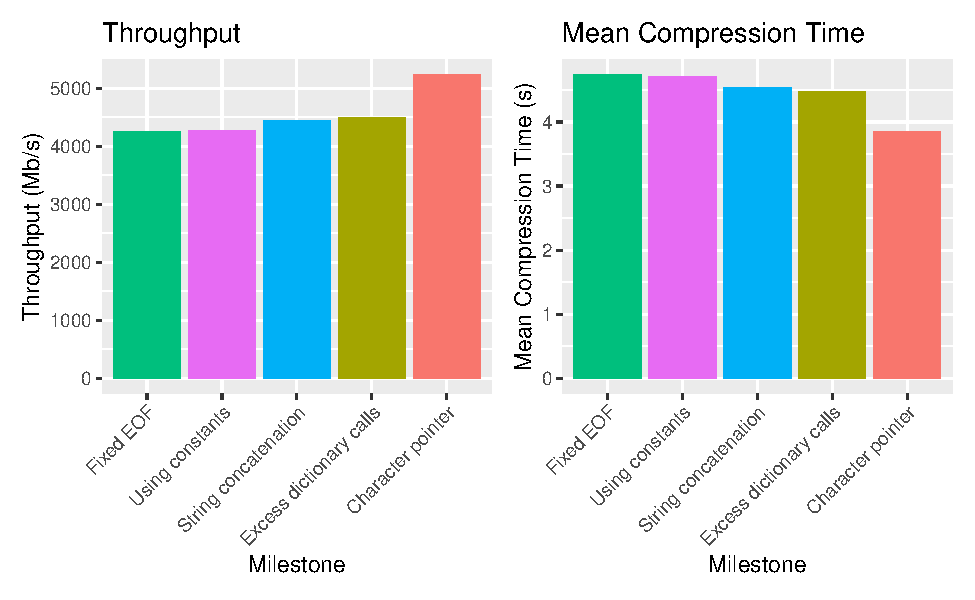
\includegraphics{thesis_files/figure-latex/comparecorporaoptimizingfig-1.pdf}
\caption{\label{fig:comparecorporaoptimizingfig}Comparison of the performance of the different milestones}
\end{figure}
\hypertarget{trying-different-dictionaries}{%
\section{Trying Different Dictionaries}\label{trying-different-dictionaries}}

A lot of the stress of the LZW algorithm is on the dictionary. We are constantly looking strings up and placing others. Because of the reliance on this data structure, we know that the dictionary accesses and lookups are a bottleneck, so improvements in those areas could greatly increase the efficiency of our program.

So the another step towards an efficient LZW seemed to be to abstract out the \texttt{std\_map} and have multiple different dictionary implementations to try and experiment with in our attempt to optimize LZW for DNA compression.

\hypertarget{direct-map}{%
\subsection{Direct Map}\label{direct-map}}

In our analysis of the two corpora, we found some interesting statistics in the redundancy of the data.

Below is a table which shows stats on the runs lengths of the ``runs'' of data, where a run is a string added to the dictionary during a run of the LZW algorithm.
\begin{table}[H]

\caption{\label{tab:runstatsfig}Run Lengths for Corpus 1}
\centering
\resizebox{\linewidth}{!}{
\begin{tabular}[t]{rrrr}
\toprule
average\_run\_length & maximum\_run\_length & median\_run\_length & sd\_run\_length\\
\midrule
\cellcolor{gray!6}{6.135398} & \cellcolor{gray!6}{17} & \cellcolor{gray!6}{6} & \cellcolor{gray!6}{1.237217}\\
\bottomrule
\end{tabular}}
\end{table}
\begin{table}[H]

\caption{\label{tab:runstatsfig}Run Lengths for Corpus 2}
\centering
\resizebox{\linewidth}{!}{
\begin{tabular}[t]{rrrr}
\toprule
average\_run\_length & maximum\_run\_length & median\_run\_length & sd\_run\_length\\
\midrule
\cellcolor{gray!6}{10.96825} & \cellcolor{gray!6}{190} & \cellcolor{gray!6}{11} & \cellcolor{gray!6}{2.494305}\\
\bottomrule
\end{tabular}}
\end{table}
And here is the combined stats of both copora, along with a histogram of all the runs.
\begin{table}[H]

\caption{\label{tab:bothrunsfig}Run lengths for both corpora}
\centering
\resizebox{\linewidth}{!}{
\begin{tabular}[t]{rrrrr}
\toprule
X & average\_run\_length & maximum\_run\_length & median\_run\_length & sd\_run\_length\\
\midrule
\cellcolor{gray!6}{1} & \cellcolor{gray!6}{10.95318} & \cellcolor{gray!6}{190} & \cellcolor{gray!6}{11} & \cellcolor{gray!6}{2.505904}\\
\bottomrule
\end{tabular}}
\end{table}
\begin{figure}
\centering
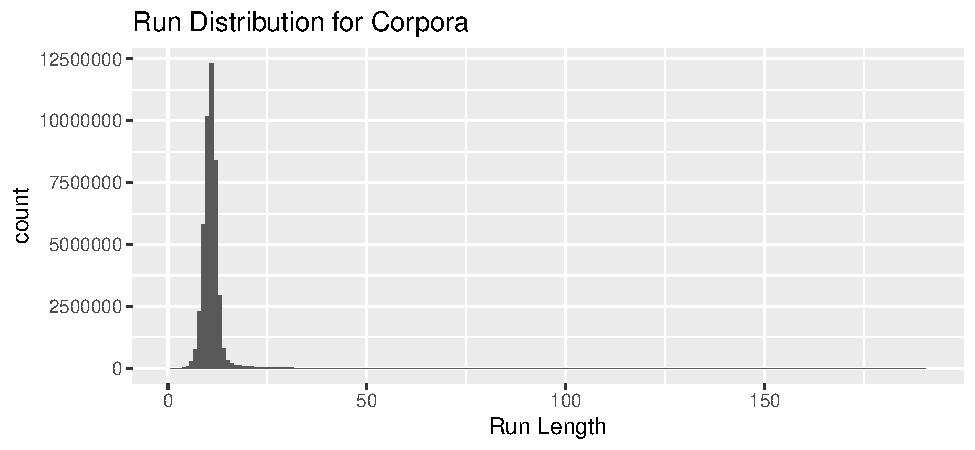
\includegraphics{thesis_files/figure-latex/allrunshistfig-1.pdf}
\caption{\label{fig:allrunshistfig}A histogram showing the lengths of runs for both copora.}
\end{figure}
Given this data, it is clear that it would be advantageous to speed up the dictionary for smaller run sizes, since most of the runs are below size 15.

To achieve this, we opted for a unique approach. Rather than use a hashmap, we can map the strings directly into memory. Since all of the strings only contain four characters (`A', `C', `T', and `G'), we can represent the characters with two bits. So for a length \texttt{n} string, we can represent it with \texttt{2n} bits.

So we can create an indexed dictionary directly in memory for all strings below a certain length. We can use the \texttt{2n} bit representation of the string
to index into an array of codewords.

For each strings size 1 to n , we have an array with enough slots for every possible string. For example, for strings of length 3, we have an array of size \(4^3\), since there are \(4^3\) possible strings. In each of those \(4^3\) slots, we have space for a codeword. All strings of length 3 can be represented by 6 bits, and since 6 bits can represent \(2^6=4^3\) values, we can use the bit representation to index into the dictionary. If the codeword at that place in the dictionary is 0, we have never seen it before. If it is non-zero, we have found the codeword for that string. For all strings greater than \texttt{n}, we can just use a hashmap on top to handle those.

Here is the data for this version of the dictionary of length 10.
\begin{table}[H]

\caption{\label{tab:directmaplength10statsfig}Corpus 1 Stats for Direct Map of max length 10}
\centering
\resizebox{\linewidth}{!}{
\begin{tabular}[t]{lrrrrr}
\toprule
File.Name & Original.File.Size & Compressed.Size & Compression.Ratio & Compression.Time & Decompression.Time\\
\midrule
\cellcolor{gray!6}{DNACorpus1/humprtb} & \cellcolor{gray!6}{56737} & \cellcolor{gray!6}{25883} & \cellcolor{gray!6}{2.192} & \cellcolor{gray!6}{1} & \cellcolor{gray!6}{2}\\
DNACorpus1/humdyst & 38770 & 18437 & 2.103 & 1 & 1\\
\cellcolor{gray!6}{DNACorpus1/vaccg} & \cellcolor{gray!6}{191737} & \cellcolor{gray!6}{77120} & \cellcolor{gray!6}{2.486} & \cellcolor{gray!6}{4} & \cellcolor{gray!6}{4}\\
DNACorpus1/hehcmv & 229354 & 93251 & 2.460 & 2 & 5\\
\cellcolor{gray!6}{DNACorpus1/mpomtcg} & \cellcolor{gray!6}{186609} & \cellcolor{gray!6}{77315} & \cellcolor{gray!6}{2.414} & \cellcolor{gray!6}{4} & \cellcolor{gray!6}{4}\\
\addlinespace
DNACorpus1/humhdab & 58864 & 26752 & 2.200 & 1 & 2\\
\cellcolor{gray!6}{DNACorpus1/chmpxx} & \cellcolor{gray!6}{121024} & \cellcolor{gray!6}{49414} & \cellcolor{gray!6}{2.449} & \cellcolor{gray!6}{3} & \cellcolor{gray!6}{3}\\
DNACorpus1/mtpacga & 100314 & 42203 & 2.377 & 2 & 2\\
\cellcolor{gray!6}{DNACorpus1/chntxx} & \cellcolor{gray!6}{155844} & \cellcolor{gray!6}{64879} & \cellcolor{gray!6}{2.402} & \cellcolor{gray!6}{3} & \cellcolor{gray!6}{3}\\
DNACorpus1/humghcs & 66495 & 29864 & 2.227 & 1 & 2\\
\addlinespace
\cellcolor{gray!6}{DNACorpus1/humhbb} & \cellcolor{gray!6}{73308} & \cellcolor{gray!6}{32681} & \cellcolor{gray!6}{2.243} & \cellcolor{gray!6}{1} & \cellcolor{gray!6}{2}\\
\bottomrule
\end{tabular}}
\end{table}
\begin{table}[H]

\caption{\label{tab:directmaplength10statsfig}Corpus 2 Stats for Direct Map of max length 10}
\centering
\resizebox{\linewidth}{!}{
\begin{tabular}[t]{lrrrrr}
\toprule
File.Name & Original.File.Size & Compressed.Size & Compression.Ratio & Compression.Time & Decompression.Time\\
\midrule
\cellcolor{gray!6}{DNACorpus2/YeMi} & \cellcolor{gray!6}{73689} & \cellcolor{gray!6}{31700} & \cellcolor{gray!6}{2.325} & \cellcolor{gray!6}{1} & \cellcolor{gray!6}{2}\\
DNACorpus2/DaRe & 62565020 & 21182510 & 2.954 & 656 & 442\\
\cellcolor{gray!6}{DNACorpus2/EnIn} & \cellcolor{gray!6}{26403087} & \cellcolor{gray!6}{8986109} & \cellcolor{gray!6}{2.938} & \cellcolor{gray!6}{271} & \cellcolor{gray!6}{184}\\
DNACorpus2/HePy & 1667825 & 572507 & 2.913 & 26 & 17\\
\cellcolor{gray!6}{DNACorpus2/OrSa} & \cellcolor{gray!6}{43262523} & \cellcolor{gray!6}{15008736} & \cellcolor{gray!6}{2.882} & \cellcolor{gray!6}{431} & \cellcolor{gray!6}{319}\\
\addlinespace
DNACorpus2/EsCo & 4641652 & 1621508 & 2.863 & 51 & 42\\
\cellcolor{gray!6}{DNACorpus2/GaGa} & \cellcolor{gray!6}{148532294} & \cellcolor{gray!6}{52441876} & \cellcolor{gray!6}{2.832} & \cellcolor{gray!6}{1475} & \cellcolor{gray!6}{1080}\\
DNACorpus2/ScPo & 10652155 & 3691943 & 2.885 & 108 & 83\\
\cellcolor{gray!6}{DNACorpus2/HaHi} & \cellcolor{gray!6}{3890005} & \cellcolor{gray!6}{1324571} & \cellcolor{gray!6}{2.937} & \cellcolor{gray!6}{51} & \cellcolor{gray!6}{32}\\
DNACorpus2/HoSa & 189752667 & 63973137 & 2.966 & 2035 & 1319\\
\addlinespace
\cellcolor{gray!6}{DNACorpus2/AeCa} & \cellcolor{gray!6}{1591049} & \cellcolor{gray!6}{561527} & \cellcolor{gray!6}{2.833} & \cellcolor{gray!6}{22} & \cellcolor{gray!6}{18}\\
DNACorpus2/DrMe & 32181429 & 11150498 & 2.886 & 332 & 237\\
\cellcolor{gray!6}{DNACorpus2/BuEb} & \cellcolor{gray!6}{18940} & \cellcolor{gray!6}{9894} & \cellcolor{gray!6}{1.914} & \cellcolor{gray!6}{0} & \cellcolor{gray!6}{1}\\
DNACorpus2/PlFa & 8986712 & 2972072 & 3.024 & 106 & 67\\
\cellcolor{gray!6}{DNACorpus2/AgPh} & \cellcolor{gray!6}{43970} & \cellcolor{gray!6}{20885} & \cellcolor{gray!6}{2.105} & \cellcolor{gray!6}{1} & \cellcolor{gray!6}{1}\\
\bottomrule
\end{tabular}}
\end{table}
Here is a comparison for different max string lengths.

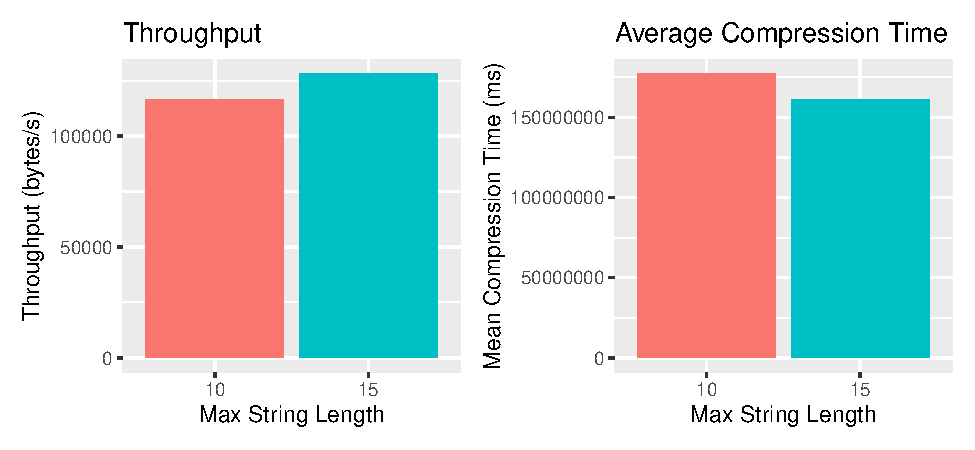
\includegraphics{thesis_files/figure-latex/directmaplenthcompfig-1.pdf}
The direct map method is very memory intensive, so having a max length over 15 is not feasible. At this point, if any runs are longer than the max string length, we just use a regular dictionary to accommodate them.

\hypertarget{multiple-indexed-dictionaries}{%
\subsection{Multiple Indexed Dictionaries}\label{multiple-indexed-dictionaries}}

As stated before, there have been research papers about the possibility of using multiple indexed dictionaries for LZW, including Keerthy (Keerthy, 2019).

Similar to the Direct Mapped approach, we use dictionaries for each string size up to a certain size \texttt{n} , and for all strings of length greater than \texttt{n}, we use a regular dictionary. As with the direct map dictionary, we need to specify a max string length. We collected metrics for different choices of max string length. Here are the results for this dictionary.
\begin{table}[H]

\caption{\label{tab:multdictlength10statsfig}Corpus 1 Stats for Multiple Dictionaries of max length 10}
\centering
\resizebox{\linewidth}{!}{
\begin{tabular}[t]{lrrrrr}
\toprule
File.Name & Original.File.Size & Compressed.Size & Compression.Ratio & Compression.Time & Decompression.Time\\
\midrule
\cellcolor{gray!6}{DNACorpus1/humprtb} & \cellcolor{gray!6}{56737} & \cellcolor{gray!6}{21687} & \cellcolor{gray!6}{2.616} & \cellcolor{gray!6}{5} & \cellcolor{gray!6}{2}\\
DNACorpus1/humdyst & 38770 & 15116 & 2.565 & 3 & 1\\
\cellcolor{gray!6}{DNACorpus1/vaccg} & \cellcolor{gray!6}{191737} & \cellcolor{gray!6}{69820} & \cellcolor{gray!6}{2.746} & \cellcolor{gray!6}{14} & \cellcolor{gray!6}{6}\\
DNACorpus1/hehcmv & 229354 & 85279 & 2.689 & 16 & 7\\
\cellcolor{gray!6}{DNACorpus1/mpomtcg} & \cellcolor{gray!6}{186609} & \cellcolor{gray!6}{70007} & \cellcolor{gray!6}{2.666} & \cellcolor{gray!6}{15} & \cellcolor{gray!6}{6}\\
\addlinespace
DNACorpus1/humhdab & 58864 & 22484 & 2.618 & 5 & 2\\
\cellcolor{gray!6}{DNACorpus1/chmpxx} & \cellcolor{gray!6}{121024} & \cellcolor{gray!6}{43269} & \cellcolor{gray!6}{2.797} & \cellcolor{gray!6}{10} & \cellcolor{gray!6}{4}\\
DNACorpus1/mtpacga & 100314 & 36647 & 2.737 & 8 & 3\\
\cellcolor{gray!6}{DNACorpus1/chntxx} & \cellcolor{gray!6}{155844} & \cellcolor{gray!6}{58089} & \cellcolor{gray!6}{2.683} & \cellcolor{gray!6}{12} & \cellcolor{gray!6}{5}\\
DNACorpus1/humghcs & 66495 & 25336 & 2.625 & 6 & 2\\
\addlinespace
\cellcolor{gray!6}{DNACorpus1/humhbb} & \cellcolor{gray!6}{73308} & \cellcolor{gray!6}{27918} & \cellcolor{gray!6}{2.626} & \cellcolor{gray!6}{7} & \cellcolor{gray!6}{2}\\
\bottomrule
\end{tabular}}
\end{table}
\begin{table}[H]

\caption{\label{tab:multdictlength10statsfig}Corpus 1 Stats for Multiple Dictionaries of max length 10}
\centering
\resizebox{\linewidth}{!}{
\begin{tabular}[t]{lrrrrr}
\toprule
File.Name & Original.File.Size & Compressed.Size & Compression.Ratio & Compression.Time & Decompression.Time\\
\midrule
\cellcolor{gray!6}{DNACorpus2/YeMi} & \cellcolor{gray!6}{73689} & \cellcolor{gray!6}{27019} & \cellcolor{gray!6}{2.727} & \cellcolor{gray!6}{7} & \cellcolor{gray!6}{2}\\
DNACorpus2/DaRe & 62565020 & 19585959 & 3.194 & 8878 & 1721\\
\cellcolor{gray!6}{DNACorpus2/EnIn} & \cellcolor{gray!6}{26403087} & \cellcolor{gray!6}{8609527} & \cellcolor{gray!6}{3.067} & \cellcolor{gray!6}{3347} & \cellcolor{gray!6}{696}\\
DNACorpus2/HePy & 1667825 & 566631 & 2.943 & 94 & 34\\
\cellcolor{gray!6}{DNACorpus2/OrSa} & \cellcolor{gray!6}{43262523} & \cellcolor{gray!6}{14147605} & \cellcolor{gray!6}{3.058} & \cellcolor{gray!6}{5551} & \cellcolor{gray!6}{1223}\\
\addlinespace
DNACorpus2/EsCo & 4641652 & 1593032 & 2.914 & 364 & 105\\
\cellcolor{gray!6}{DNACorpus2/GaGa} & \cellcolor{gray!6}{148532294} & \cellcolor{gray!6}{46851235} & \cellcolor{gray!6}{3.170} & \cellcolor{gray!6}{22817} & \cellcolor{gray!6}{4323}\\
DNACorpus2/ScPo & 10652155 & 3590421 & 2.967 & 1099 & 258\\
\cellcolor{gray!6}{DNACorpus2/HaHi} & \cellcolor{gray!6}{3890005} & \cellcolor{gray!6}{1306336} & \cellcolor{gray!6}{2.978} & \cellcolor{gray!6}{302} & \cellcolor{gray!6}{86}\\
DNACorpus2/HoSa & 189752667 & 57199679 & 3.317 & 31978 & 5449\\
\addlinespace
\cellcolor{gray!6}{DNACorpus2/AeCa} & \cellcolor{gray!6}{1591049} & \cellcolor{gray!6}{556194} & \cellcolor{gray!6}{2.861} & \cellcolor{gray!6}{91} & \cellcolor{gray!6}{34}\\
DNACorpus2/DrMe & 32181429 & 10618575 & 3.031 & 3865 & 905\\
\cellcolor{gray!6}{DNACorpus2/BuEb} & \cellcolor{gray!6}{18940} & \cellcolor{gray!6}{7740} & \cellcolor{gray!6}{2.447} & \cellcolor{gray!6}{1} & \cellcolor{gray!6}{0}\\
DNACorpus2/PlFa & 8986712 & 2895340 & 3.104 & 892 & 211\\
\cellcolor{gray!6}{DNACorpus2/AgPh} & \cellcolor{gray!6}{43970} & \cellcolor{gray!6}{17258} & \cellcolor{gray!6}{2.548} & \cellcolor{gray!6}{4} & \cellcolor{gray!6}{1}\\
\bottomrule
\end{tabular}}
\end{table}
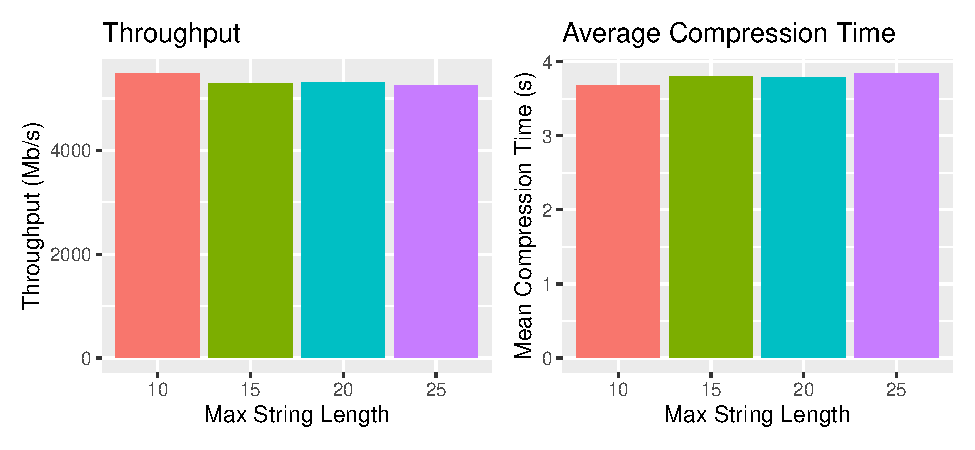
\includegraphics{thesis_files/figure-latex/multdictlengthcompfig-1.pdf}
Here is a comparison of the Multiple Dictionaries versus one standard dictionary.
\begin{figure}
\centering
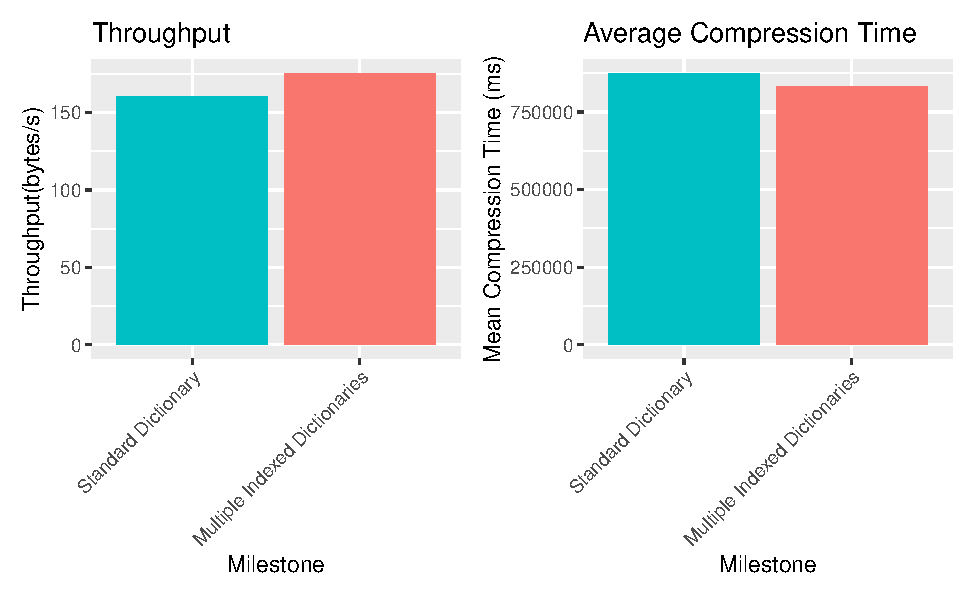
\includegraphics{thesis_files/figure-latex/multvsonedictfig-1.pdf}
\caption{\label{fig:multvsonedictfig}Comparing one Dict to Mult Dict}
\end{figure}
\hypertarget{comparison}{%
\subsection{Comparison}\label{comparison}}

Here is a comparison of all three techniques: Standard Dictionary, Multiple Standard Dictionaries, and Direct Mapped Dictionary.
\begin{figure}
\centering
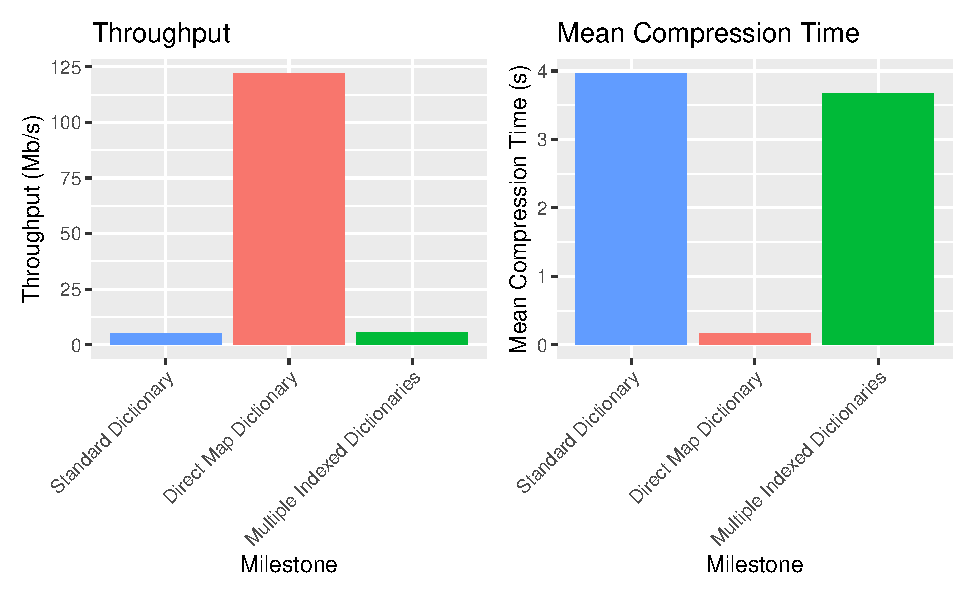
\includegraphics{thesis_files/figure-latex/dictionarytechniquecompfig-1.pdf}
\caption{\label{fig:dictionarytechniquecompfig}Comparing the three types of dictionaries. The Direct Map has a max length of 15 and the Mult Dict has a max length of 10.}
\end{figure}
\hypertarget{optimizing-direct-map-even-more}{%
\section{Optimizing Direct Map Even more}\label{optimizing-direct-map-even-more}}

Since the Direct map dictionary was a standout in performance, we decided to focus on optimizing it even further.

\hypertarget{finding-the-longest-runs}{%
\subsection{Finding the Longest Runs}\label{finding-the-longest-runs}}

Our dictionary data structures all have a \texttt{get\_longest\_in\_dict} function. This function does the boring work of iterating through the input from the start, checking if each substring is in the dictionary.

Given the statistics of our corpora, we know that this process can be faster. Since most runs are above 6-7, we waste a lot of time by starting from the bottom.

Another strategy would be to start from the maximum string length of the dictionary. We can check if the next string of the max length in the dictionary. If it is, we need to check strings longer than the max, so we can iterate up. If it isn't, we need to check strings shorter, so we can either iterate down or binary search down from the max. Here is a table showing the performance of these different strategies.
\begin{figure}
\centering
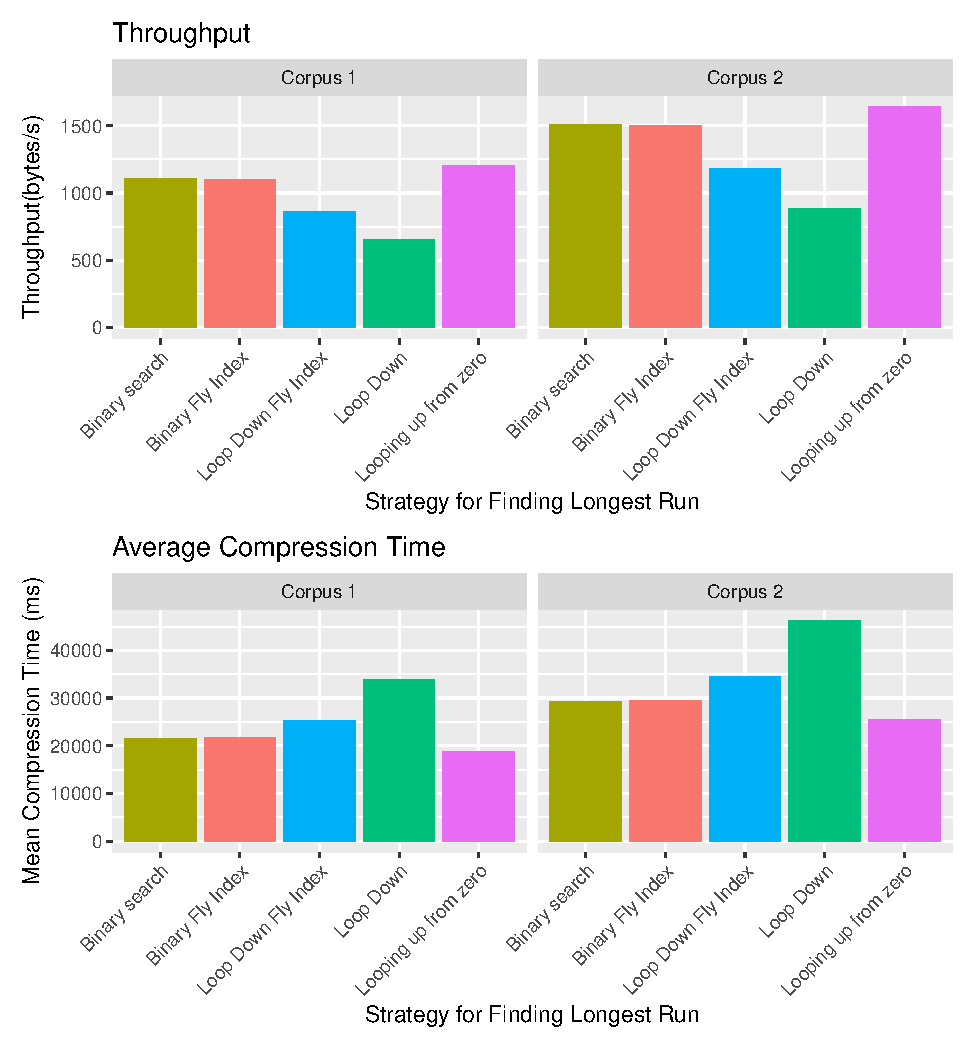
\includegraphics{thesis_files/figure-latex/findlongestfrommaxfig-1.pdf}
\caption{\label{fig:findlongestfrommaxfig}Comparing the different ways of finding the longest run}
\end{figure}
We see that none of the other strategies are better than just looping up from zero. This could be because most of the runs are very short, which we can see in \ref{fig:allrunshistfig}. This means that if we start looking from runs around length 10, we should see a performance improvement.

\hypertarget{finding-the-longest-from-the-average}{%
\subsection{Finding the Longest From The Average}\label{finding-the-longest-from-the-average}}

Here are the results when we try looking for runs starting at the average.
\begin{figure}
\centering
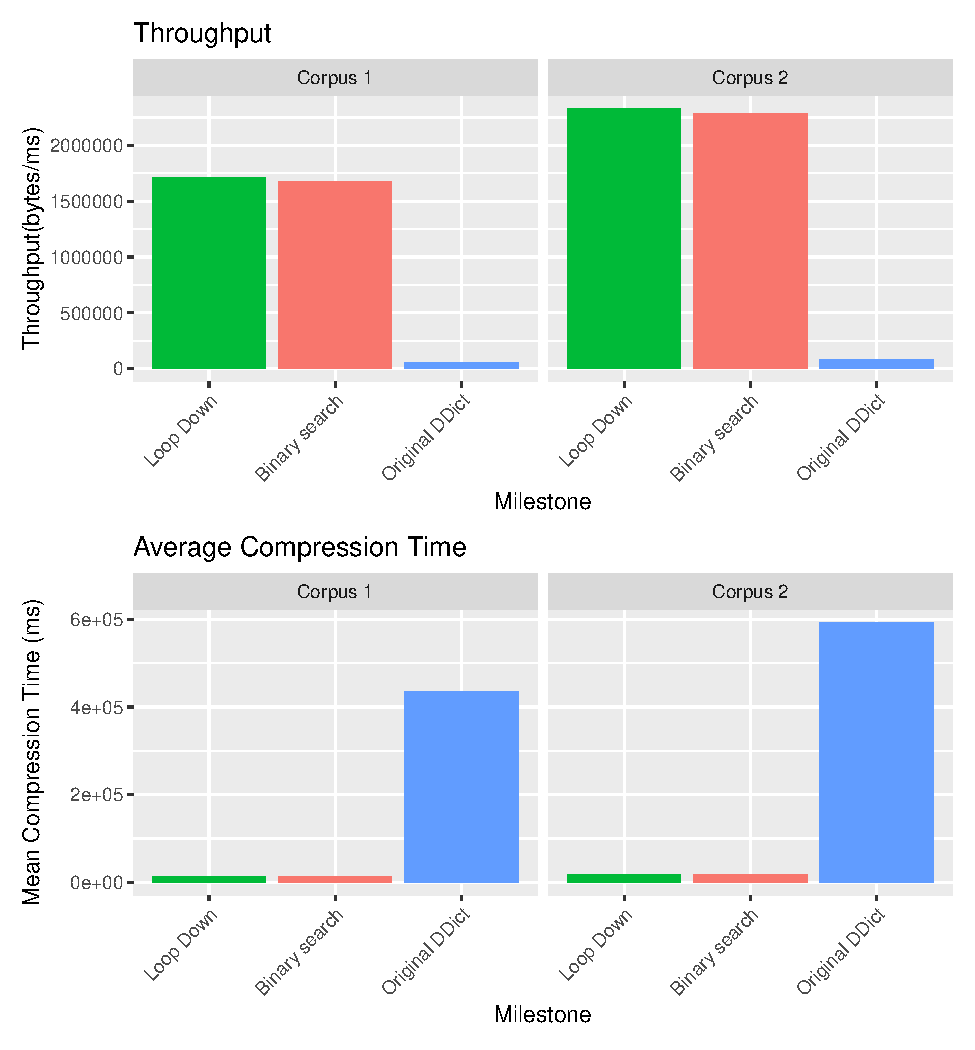
\includegraphics{thesis_files/figure-latex/findlongestfromavg-1.pdf}
\caption{\label{fig:findlongestfromavg}Comparing the different ways of finding the longest run}
\end{figure}
As we predicted, this greatly improves performance. We are capitalizing on the fact that most runs are short. There is the occasional run that is very long, but from the run statistics we saw that the standard deviation for both corpora was pretty small. So on the edge cases in which there are very long runs, we could be wasting a lot of time.

\hypertarget{not-allowing-strings-over-max}{%
\subsection{Not Allowing strings over max}\label{not-allowing-strings-over-max}}

One way to avoid the edge case where we encounter a very long run is to just not allow strings in the dictionary longer than the max string length, in this case, 15. This means we won't have to deal with the overhead of the hashmap on top of our dictionary, but we will take a hit in compression ratio.

Here is a graph comparing the different strategies.

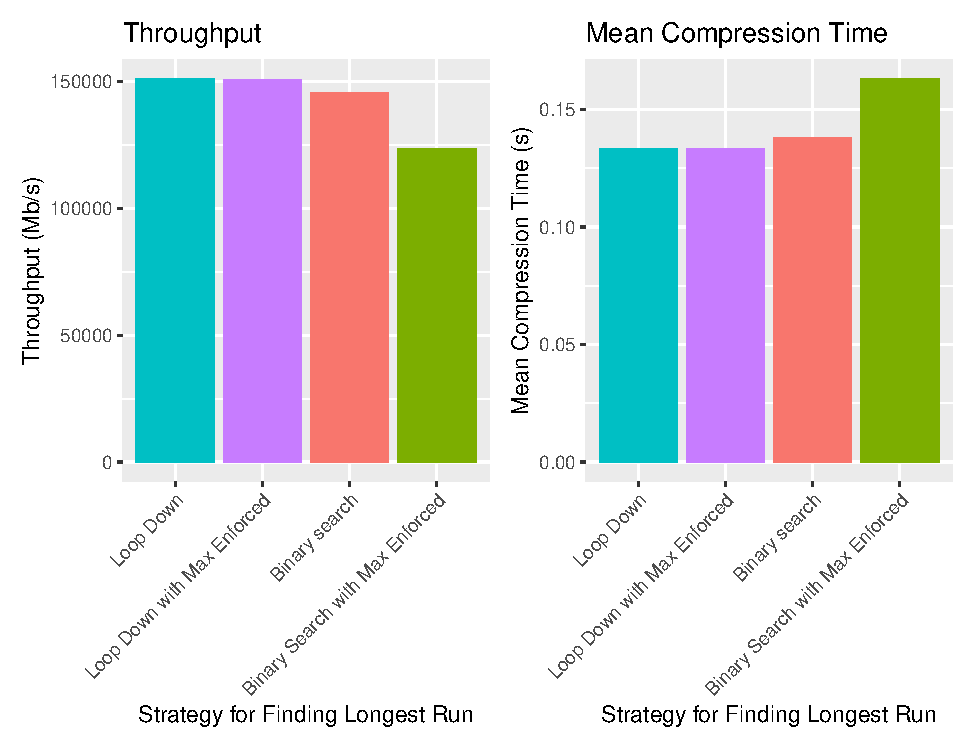
\includegraphics{thesis_files/figure-latex/findlongestwmax-1.pdf}
There isn't too much of a performance improvement, which makes sense because long runs are very rare. Let's see how it affects our compression ratio.
\begin{table}[H]

\caption{\label{tab:maxenforcedstats}Compression Ratio change from disallowing long strings}
\centering
\resizebox{\linewidth}{!}{
\begin{tabular}[t]{rr}
\toprule
cr\_before & cr\_after\\
\midrule
\cellcolor{gray!6}{2.909175} & \cellcolor{gray!6}{2.907686}\\
\bottomrule
\end{tabular}}
\end{table}
The effect on the total compression ratio is minimal

\hypertarget{using-pext}{%
\subsection{\texorpdfstring{Using \texttt{pext}}{Using pext}}\label{using-pext}}

One potential bottleneck of finding the longest run is converting a run of characters into an index. We can try to do it on the fly as we loop up or down, but we could also use machine instructions.

Our strategy is to use \texttt{pext}, which extracts parallel bits. We give \texttt{pext} a string of characters, say `ACTG', and a bit mask, and it will extract those bits from our string. It theoretically does this in one machine instruction, which could be much more efficient than looping over all the characters.
\begin{figure}
\centering
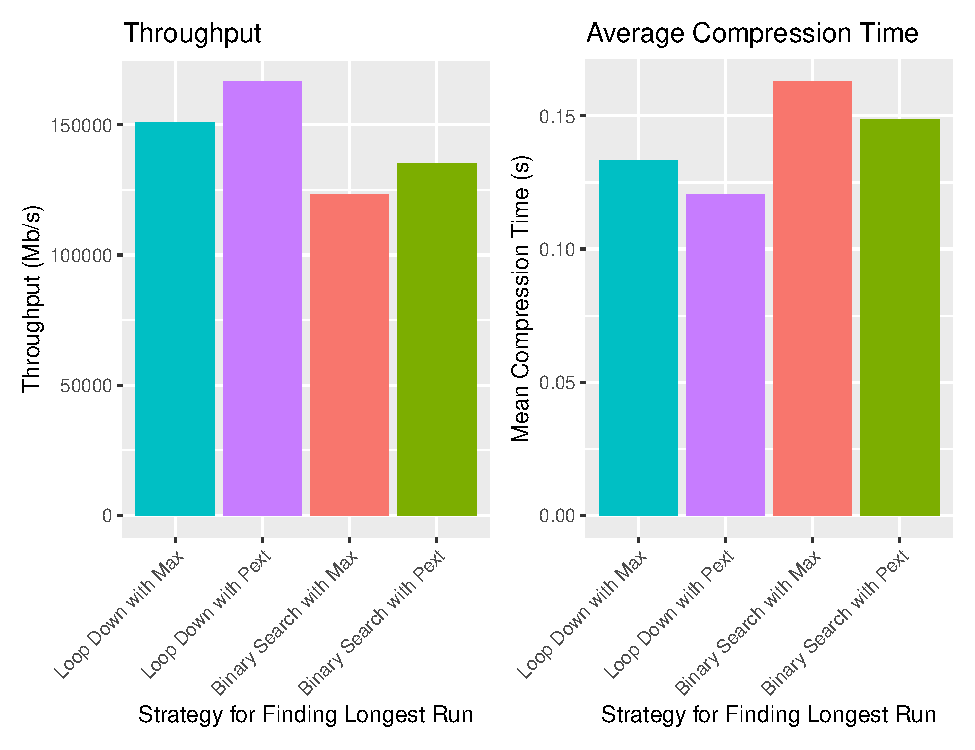
\includegraphics{thesis_files/figure-latex/findlongestwpext-1.pdf}
\caption{\label{fig:findlongestwpext}Comparing the different ways of finding the longest run with pext}
\end{figure}
Why doesn't it work?

\hypertarget{comparison-to-other-tools}{%
\chapter{Comparison to other tools}\label{comparison-to-other-tools}}

Here, in this chapter, we will investigate how our implementation holds up against other compression methods.

\hypertarget{conclusion}{%
\chapter*{Conclusion}\label{conclusion}}
\addcontentsline{toc}{chapter}{Conclusion}

If we don't want Conclusion to have a chapter number next to it, we can add the \texttt{\{-\}} attribute.

\textbf{More info}

And here's some other random info: the first paragraph after a chapter title or section head \emph{shouldn't be} indented, because indents are to tell the reader that you're starting a new paragraph. Since that's obvious after a chapter or section title, proper typesetting doesn't add an indent there.

\appendix

\hypertarget{the-first-appendix}{%
\chapter{The First Appendix}\label{the-first-appendix}}

This first appendix includes all of the R chunks of code that were hidden throughout the document (using the \texttt{include\ =\ FALSE} chunk tag) to help with readibility and/or setup.

\textbf{In the main Rmd file}
\begin{Shaded}
\begin{Highlighting}[]
\CommentTok{\# This chunk ensures that the thesisdown package is}
\CommentTok{\# installed and loaded. This thesisdown package includes}
\CommentTok{\# the template files for the thesis.}
\ControlFlowTok{if}\NormalTok{ (}\SpecialCharTok{!}\FunctionTok{require}\NormalTok{(remotes)) \{}
  \ControlFlowTok{if}\NormalTok{ (params}\SpecialCharTok{$}\StringTok{\textasciigrave{}}\AttributeTok{Install needed packages for \{thesisdown\}}\StringTok{\textasciigrave{}}\NormalTok{) \{}
    \FunctionTok{install.packages}\NormalTok{(}\StringTok{"remotes"}\NormalTok{, }\AttributeTok{repos =} \StringTok{"https://cran.rstudio.com"}\NormalTok{)}
\NormalTok{  \} }\ControlFlowTok{else}\NormalTok{ \{}
    \FunctionTok{stop}\NormalTok{(}
      \FunctionTok{paste}\NormalTok{(}\StringTok{\textquotesingle{}You need to run install.packages("remotes")",}
\StringTok{            "first in the Console.\textquotesingle{}}\NormalTok{)}
\NormalTok{    )}
\NormalTok{  \}}
\NormalTok{\}}
\ControlFlowTok{if}\NormalTok{ (}\SpecialCharTok{!}\FunctionTok{require}\NormalTok{(thesisdown)) \{}
  \ControlFlowTok{if}\NormalTok{ (params}\SpecialCharTok{$}\StringTok{\textasciigrave{}}\AttributeTok{Install needed packages for \{thesisdown\}}\StringTok{\textasciigrave{}}\NormalTok{) \{}
\NormalTok{    remotes}\SpecialCharTok{::}\FunctionTok{install\_github}\NormalTok{(}\StringTok{"ismayc/thesisdown"}\NormalTok{)}
\NormalTok{  \} }\ControlFlowTok{else}\NormalTok{ \{}
    \FunctionTok{stop}\NormalTok{(}
      \FunctionTok{paste}\NormalTok{(}
        \StringTok{"You need to run"}\NormalTok{,}
        \StringTok{\textquotesingle{}remotes::install\_github("ismayc/thesisdown")\textquotesingle{}}\NormalTok{,}
        \StringTok{"first in the Console."}
\NormalTok{      )}
\NormalTok{    )}
\NormalTok{  \}}
\NormalTok{\}}
\FunctionTok{library}\NormalTok{(thesisdown)}
\ControlFlowTok{if}\NormalTok{ (}\SpecialCharTok{!}\FunctionTok{require}\NormalTok{(DiagrammeR)) \{}
  \FunctionTok{install.packages}\NormalTok{(}\StringTok{"DiagrammeR"}\NormalTok{)}
\NormalTok{\}}
\FunctionTok{library}\NormalTok{(DiagrammeR)}
\CommentTok{\# Set how wide the R output will go}
\FunctionTok{options}\NormalTok{(}\AttributeTok{width =} \DecValTok{70}\NormalTok{)}
\end{Highlighting}
\end{Shaded}
\textbf{In Chapter \ref{ref-labels}:}

\hypertarget{the-second-appendix-for-fun}{%
\chapter{The Second Appendix, for Fun}\label{the-second-appendix-for-fun}}

\backmatter

\hypertarget{references}{%
\chapter*{References}\label{references}}
\addcontentsline{toc}{chapter}{References}

\markboth{References}{References}

\noindent

\setlength{\parindent}{-0.20in}
\begin{verbatim}
Huffman, D. A. (1952). A method for the construction of minimum-redundancy codes. Proceedings of the IRE, 40(9), 1098-1101.
Sayood, K. (2017). Introduction to data compression. Academic Press.
Witten, I. H., Neal, R. M., & Cleary, J. G. (1987). Arithmetic coding for data compression. Communications of the ACM, 30(6), 520-540.
Sayood, K. (2017). Introduction to data compression. Academic Press.
Pratas, Diogo & Pinho, Armando. (2018). A DNA Sequence Corpus for Compression Benchmark. 208-215. 10.1007/978-3-319-98702-6_25.
\end{verbatim}
\hypertarget{refs}{}
\begin{CSLReferences}{1}{0}
\leavevmode\vadjust pre{\hypertarget{ref-angel2000}{}}%
Angel, E. (2000). \emph{Interactive computer graphics : A top-down approach with OpenGL}. Boston, MA: Addison Wesley Longman.

\leavevmode\vadjust pre{\hypertarget{ref-angel2001}{}}%
Angel, E. (2001a). \emph{Batch-file computer graphics : A bottom-up approach with QuickTime}. Boston, MA: Wesley Addison Longman.

\leavevmode\vadjust pre{\hypertarget{ref-angel2002a}{}}%
Angel, E. (2001b). \emph{Test second book by angel}. Boston, MA: Wesley Addison Longman.

\leavevmode\vadjust pre{\hypertarget{ref-grumbach}{}}%
Grumbach, S., \& Tahi, F. (1994). {A New Challenge for Compression Algorithms: Genetic Sequences}. \emph{{Information Processing and Management}}, \emph{30}. Retrieved from \url{https://hal.inria.fr/inria-00180949}

\leavevmode\vadjust pre{\hypertarget{ref-ibrahimgbolagade}{}}%
Ibrahim, M., \& Gbolagade, K. (2020). Enhancing computational time of lempel-ziv-welch-based text compression with chinese remainder theorem. \emph{Journal of Computer Science and Its Application}, \emph{27}. http://doi.org/\href{https://doi.org/10.4314/jcsia.v27i1.9}{10.4314/jcsia.v27i1.9}

\leavevmode\vadjust pre{\hypertarget{ref-KeerthyMID}{}}%
Keerthy, P. (2019). Genomic sequence data compression using lempel-ziv-welch algorithm with indexed multiple dictionary. \emph{International Journal of Engineering and Advanced Technology}.

\leavevmode\vadjust pre{\hypertarget{ref-panialok}{}}%
Pani, A., Mishra, M., \& Mishra, T. (2012). Parallel lempel-ziv-welch (PLZW) technique for data compression. \emph{International Journal of Computer Science and Information Technology}, \emph{3}, 4038--4040.

\leavevmode\vadjust pre{\hypertarget{ref-prataspinho}{}}%
Pratas, D., \& Pinho, A. (2018). A DNA sequence corpus for compression benchmark. In (pp. 208--215). http://doi.org/\href{https://doi.org/10.1007/978-3-319-98702-6_25}{10.1007/978-3-319-98702-6\_25}

\end{CSLReferences}

% Index?

\end{document}
